%! Author = Omar Iskandarani
%! Title = Swirl String Theory (SST) Canon v0.7
%! Date = Dec 26, 2025
%! Affiliation = Independent Researcher, Groningen, The Netherlands
%! License = © 2025 Omar Iskandarani. All rights reserved. This manuscript is made available for academic reading and citation only. No republication, redistribution, or derivative works are permitted without explicit written permission from the author. Contact: info@omariskandarani.com
%! ORCID = 0009-0006-1686-3961
%! DOI = 10.5281/zenodo.18233522

\newcommand{\canonversion}{v0.7.7} % Semantic versioning: vMAJOR.MINOR.PATCH
\newcommand{\papertitle}{\textbf{Swirl String Theory (SST) Canon \canonversion:} \\
                         \Large Quantum Measurement, Time, Gravity, and Atomic Mass\\ from Topological Defects}
\newcommand{\paperdoi}{10.5281/zenodo.18233522}

%========================================================================================
% PACKAGES AND DOCUMENT CONFIGURATION
%========================================================================================
\documentclass[10pt]{article}

% ====== minimal packages ======

\usepackage[utf8]{inputenc}
\usepackage[T1]{fontenc}
\usepackage{amsmath, amssymb, amsfonts}
\usepackage{geometry}
\usepackage{graphicx}
\usepackage{hyperref}
\usepackage{physics}
\usepackage{xcolor}
\usepackage{textcomp}
\usepackage{amsthm}

\usepackage{bm}
\usepackage{microtype}
\usepackage{tcolorbox}
\hypersetup{colorlinks=true,linkcolor=blue,citecolor=blue,urlcolor=blue}

% ==== Packages ====
\usepackage{lmodern}
\usepackage{booktabs}
\usepackage{tikz}
\usetikzlibrary{arrows.meta,positioning,calc,fit,decorations.pathmorphing}
% Tables and Figures
\usepackage{float}
\usepackage{import}
\usepackage{tabularx}
\usepackage{enumitem}
% ==========================
% PATCH 0: include utilities
% ==========================
\usepackage{appendix}

\usepackage{setspace}

% ==========================
% PATCH 0b: theorem-like envs
% ==========================
\newtheorem{definition}{Definition}[section]
\newtheorem{proposition}{Proposition}[section]
\newtheorem{remark}{Remark}[section]

% Page geometry
\geometry{top=2.5cm, bottom=2.5cm, left=2.5cm, right=2.5cm}

% Hyperlink setup
\hypersetup{
    colorlinks=true,
    linkcolor=blue,
    citecolor=red,
    urlcolor=blue
}

% ===== Gauge sector macros =====
\providecommand{\Tr}{\mathrm{Tr}}
\newcommand{\ii}{\mathrm{i}}
% Gauge fields (adjoints; indices a=1..8, i=1..3)
\newcommand{\GsA}{G^a_{\mu\nu}}
\newcommand{\WsI}{W^i_{\mu\nu}}
\newcommand{\Bmn}{B_{\mu\nu}}
\sloppy
% ===============================
% Macros (canonicalized)
% ===============================
%=== SST macros (minimal set for this snippet) =========================

% swirl arrows (context-aware)
\newcommand{\swirlarrow}{ \mathchoice{\mkern-2mu\scriptstyle\boldsymbol{\circlearrowleft}}{\mkern-2mu\scriptscriptstyle\boldsymbol{\circlearrowleft}}}
\newcommand{\vswirl}{\mathbf{v}_{\!\boldsymbol{\circlearrowleft}}}
\newcommand{\SwirlClock}{S_{(t)}^{\swirlarrow}}
\newcommand{\Fmaxswirl}{F^{\max}_{\mkern-1mu\scriptscriptstyle\boldsymbol{\circlearrowleft}}}
% swirl arrows Counter Clockwise
\newcommand{\swirlarrowcw}{ \mathchoice{\mkern-2mu\scriptstyle\boldsymbol{\circlearrowright}}{\mkern-2mu\scriptscriptstyle\boldsymbol{\circlearrowright}}}
\newcommand{\vswirlcw}{\mathbf{v}_{\swirlarrowcw}}
\newcommand{\SwirlClockcw}{S_{(t)}^{\swirlarrowcw}}
\newcommand{\Fmaxswirlcw}{F^{\max}_{\mkern-1mu\scriptscriptstyle\boldsymbol{\circlearrowright}}}

\newcommand{\Fmax}{\Fmaxswirl} % default maximal force (left swirl)
\newcommand{\FmaxEM}{F^{\max}_{\mathrm{EM}}}
\newcommand{\FmaxG}{F_{\mathrm{G}}^{\max}}               % G-like maximal force scale

\newcommand{\omegas}{\boldsymbol{\omega}_{\swirlarrow}}  % swirl vorticity
\newcommand{\Om}{\Omega_{\swirlarrow}}                   % swirl angular frequency profile

\newcommand{\vscore}{v_{\swirlarrow}}                    % shorthand: |v_swirl| at r=r_c
\newcommand{\vnorm}{\lVert \mathbf{v}_{\mkern-2mu\scriptscriptstyle\boldsymbol{\circlearrowleft}} \rVert}               % swirl speed magnitude
\newcommand{\Ce}{\vswirl}                                % canonical swirl-speed constant


\newcommand{\rhof}{\rho_{\!f}}                           % effective fluid density
\newcommand{\rhoF}{\rho_{\!f}}
\newcommand{\rhoE}{\rho_{\!E}}                           % swirl energy density
\newcommand{\rhom}{\rho_{\!m}}                           % mass-equivalent density
\newcommand{\rhoM}{\rho_{\!m}}     % mass-equivalent density
\newcommand{\rc}{r_c}                                    % string core radius (swirl string radius)

\newcommand{\Lam}{\Lambda}                               % Swirl Coulomb constant
\newcommand{\alpg}{\alpha_g}                             % gravitational fine-structure analogue

\newcommand{\Golden}{\phi}
\newcommand{\GoldenSq}{\phi^{2}}


% Status tags (house style)
\newcommand{\statusResearch}{\textsf{[Research-track]}}
\newcommand{\statusCalibration}{\textsf{[Calibration]}}
\newcommand{\statusCanonical}{\textsf{[Canonical clarification]}}

\newcommand{\omegaVec}{\boldsymbol{\omega}}

\newcommand{\OmegaCore}{\Omega_{\mathrm{core}}}
\newcommand{\bg}{\mathrm{bg}}
\newcommand{\core}{\mathrm{core}}
\newcommand{\Vol}{\operatorname{Vol}}   % now \Vol_{\!\mathbb{H}}(K) works

% ===============================
% Policy: the golden constant is only allowed via hyperbolic functions.
\newcommand{\xig}{\operatorname{asinh}\!\left(\tfrac{1}{2}\right)}
\newcommand{\phig}{\exp(\xig)}
\newcommand{\phialg}{\bigl(1+\sqrt{5}\bigr)/2}
\newcommand{\xigold}{\tfrac{3}{2}\,\xig}
\newcommand{\GoldenDeclare}{%
    \textbf{Golden (hyperbolic)}:\ \(\ln\phi=\xig\), hence \(\phi=\phig\).
    \ \emph{(Algebraic form \(\phi=\phialg\) is equivalent.)}%
}

\newcommand{\vswirltext}{\mathbf{v}_{\mathrm{swirl}}}

% ----------------------------------------------------------------------
% Operator notation (compact hydrodynamic operators; v0.7.6 patch)
% ----------------------------------------------------------------------
\newcommand{\OpOmega}{\hat{\Omega}} % vorticity operator
\newcommand{\OpPi}{\hat{\Pi}}       % advective / momentum-flux operator
\newcommand{\curlop}{\nabla\times}
\newcommand{\gradop}{\nabla}
\newcommand{\divop}{\nabla\cdot}

% TOC Customization
\usepackage{tocloft}
\usepackage{calc}
\usepackage{siunitx} % for \settowidth

\setcounter{tocdepth}{1}

% Fonts
\renewcommand{\cftsecfont}{\scriptsize}
\renewcommand{\cftsubsecfont}{\scriptsize\itshape}
\renewcommand{\cftsecpagefont}{\scriptsize}
\renewcommand{\cftsubsecpagefont}{\scriptsize}

% Dots
\renewcommand{\cftsecleader}{\cftdotfill{\cftdotsep}}
\renewcommand{\cftdotsep}{4}

% Ensure a visible gap after the number
\renewcommand{\cftsecaftersnum}{\hspace{0.9em}}
\renewcommand{\cftsubsecaftersnum}{\hspace{0.9em}}

% Reserve enough number width for the largest Roman numeral you use
% (adjust XXXVIII if you go beyond 38)
\newlength{\tocnumw}
\settowidth{\tocnumw}{\scriptsize XXXVIII\hspace{0.9em}}
\setlength{\cftsecnumwidth}{\tocnumw}
\setlength{\cftsubsecindent}{\tocnumw}
\setlength{\cftsubsecnumwidth}{\tocnumw}

% Compact TOC macro (hard-compact)
\newcommand{\compacttoc}{%
    \begingroup
    % Force font size + line spacing explicitly (this is the real vertical fix)
    \fontsize{8}{9}\selectfont % try {7.6}{8.4} if you want even tighter

    % No paragraph/list spacing inside TOC
    \setlength{\parskip}{0pt}%
    \setlength{\parindent}{0pt}%
    \setlength{\cftparskip}{0pt}%

    % Remove extra vskips inserted by tocloft
    \setlength{\cftbeforesecskip}{0pt}%
    \setlength{\cftbeforesubsecskip}{0pt}%

    % Optional: tighten title spacing if "Contents" creates whitespace
    \setlength{\cftbeforetoctitleskip}{0pt}%
    \setlength{\cftaftertoctitleskip}{4pt}%

    \tableofcontents
    \endgroup
}
% Compact list defaults (front page)
\newlist{canonlist}{enumerate}{1}
\setlist[canonlist]{label=\textbf{\Roman*.}, leftmargin=*, itemsep=2pt, topsep=2pt, parsep=0pt}

% Box style for frontpage blocks
\tcbset{
    canonfront/.style={
        colback=white,
        colframe=black!45,
        boxrule=0.5pt,
        arc=1.2mm,
        left=6pt,right=6pt,top=6pt,bottom=6pt,
    }
}


% Misc
\providecommand{\dd}{\mathrm{d}}
\newcommand{\ee}{\mathrm{e}}
\newcommand{\rhocore}{\rho_{\text{core}}}
\newcommand{\clockfield}{\chi(x)}
\newcommand{\swirlfactor}{S_\circ(x)}


\newcommand{\titlepageOpen}{
    \begin{titlepage}
    \thispagestyle{empty}
    \centering
    \Large \bfseries \papertitle \par \vspace{1cm}
    {\Large \itshape \textbf{Omar Iskandarani}\textsuperscript{\textbf{*}} \par}
    \vspace{0.5cm}
    {\today \par}
    \vspace{0.5cm}
}

\newcommand{\titlepageClose}{
    \vfill \raggedright \null
    \begin{picture}(0,0)
    \put(0,-45){  % Shift 200pt left, 40pt down
        \begin{minipage}[b]{0.7\textwidth} \footnotesize
        \renewcommand{\arraystretch}{1.0}
        \noindent\rule{\textwidth}{0.4pt} \\[0.5em]
        \textsuperscript{\textbf{*}} Independent Researcher, Groningen, The Netherlands \\
        Email: \texttt{info@omariskandarani.com} \\
        ORCID: \texttt{\href{https://orcid.org/0009-0006-1686-3961}{0009-0006-1686-3961}} \\
        DOI: \href{https://doi.org/\paperdoi}{\paperdoi}
        \end{minipage}
    }
    \end{picture}
    \end{titlepage}
}


\begin{document}
    \titlepageOpen
    \begin{abstract}

        \noindent We present Version 0.7.6 of the Swirl-String Theory (SST) Canon. This release unifies three historically distinct phenomena---time, gravity, and mass---into a single hydrodynamic framework based on a frictionless, incompressible superfluid condensate. We resolve the "Problem of Time" in quantum mechanics by defining time as a relational observable (event count) derived from a conserved topological current $J^\mu$. We demonstrate that the scalar field mediating this clock synchronization satisfies a Poisson equation, naturally yielding the inverse-square law for gravity without assuming curved spacetime. Finally, we derive the invariant masses of stable particles (protons, electrons) as the integrated swirl energy of topological knots, strictly enforcing the separation between the vacuum fluid density ($\rho_f \sim 10^{-7}$ kg/m$^3$) and the core condensate density ($\rho_{\text{core}} \sim 10^{18}$ kg/m$^3$).

    \end{abstract}
    \vspace{0.6em}

    \begin{minipage}{0.92\textwidth}
        \scriptsize
        \begin{tcolorbox}[canonfront,title={This version canonizes the following principles}]
            \begin{canonlist}
                \item The foundational hydrodynamic laws, including the Chronos--Kelvin invariant and the Swirl Coulomb constant $\Lambda$.
                \item The Swirl--Electromagnetic bridge, linking swirl dynamics directly to Maxwell-type structure.
                \item Emergence of the $\mathrm{SU}(3)\times\mathrm{SU}(2)\times\mathrm{U}(1)$ gauge sector and a first-principles derivation of the weak mixing angle $\theta_W$.
                \item A parameter-free prediction track for the electroweak symmetry breaking scale (EWSB sector statement).
                \item A formal dynamical rule for quantum measurement via $R\leftrightarrow T$ phase transitions.
            \end{canonlist}
        \end{tcolorbox}
    \end{minipage}

    \vspace{0.6em}

    \begin{minipage}{0.92\textwidth}
        \scriptsize
        \begin{tcolorbox}[canonfront,title={Core Axioms (SST)}]
            \renewcommand{\arraystretch}{1.15}
            \begin{tabularx}{\textwidth}{@{}r@{\quad}X@{}}
                \textbf{1.} & \textbf{Swirl Medium:} Physics is formulated on $\mathbb{R}^3$ with absolute reference time. Dynamics occur in a frictionless, incompressible swirl condensate.\\
                \textbf{2.} & \textbf{Swirl Strings (Circulation and Topology):} Particles and field quanta correspond to closed filamentary defects (swirl strings). Circulation is quantized:
                \[
                    \Gamma=\oint \mathbf{v}_{\!\boldsymbol{\circlearrowleft}}\cdot d\boldsymbol{\ell}=n\,\Gamma_0,\qquad
                    \Gamma_0=2\pi r_c \,\lVert \mathbf{v}_{\!\boldsymbol{\circlearrowleft}}\rVert .
                \]
                Discrete quantum numbers track to topological invariants of the swirl string.\\
                \textbf{3.} & \textbf{String-induced gravitation:} Macroscopic attraction emerges from coherent swirl flows and swirl-pressure gradients. The effective gravitational coupling is fixed by canonical constants.\\
                \textbf{4.} & \textbf{Swirl Clocks:} Local proper-time rate depends on tangential swirl speed $v$, with factor $S_t=\sqrt{1-v^2/c^2}$.\\
                \textbf{5.} & \textbf{Dual Phases (Wave--Particle):} Each swirl string admits an extended $R$-phase and a localized $T$-phase; measurement is a dynamical transition between them.\\
                \textbf{6.} & \textbf{Taxonomy:} Unknotted excitations correspond to bosonic modes; torus knots map to leptonic candidates; chiral hyperbolic knots map to quark-like candidates; linked structures map to nuclei and bound states.\\
            \end{tabularx}
        \end{tcolorbox}
    \end{minipage}
        \titlepageClose
        \newpage

        \singlespacing

        %\tableofcontents
        \compacttoc
        \newpage
% ======================================================================
    \section*{Canonical Definitions, Primitive Constants, and Operators}
    \addcontentsline*{toc}{section}{Canonical Definitions, Primitive Constants, and Operators}
% ======================================================================

\begin{definition}[Primitive constant triplet]
The \emph{zero-parameter generating set} of the hydrodynamic sector is the ordered triplet
\begin{equation}
(\Gamma_0,\ \rho_{\!f},\ r_c),
\end{equation}
where $r_c$ is the core radius, $\rho_{\!f}$ is the effective background density of the swirl medium,
and $\Gamma_0$ is the primitive circulation quantum.
\end{definition}

\paragraph{Primitive circulation quantum.}
\begin{equation}
\Gamma_0 \;\equiv\; 2\pi r_c\,\lVert \mathbf{v}_{\!\boldsymbol{\circlearrowleft}}\rVert.
\end{equation}

\paragraph{Clock / gravity / phase field.}
\begin{equation}
\chi(x)\equiv \text{scalar foliation field governing local time, gravity, and phase reference}.
\end{equation}

\paragraph{Compact differential operators.}
\begin{align}
\hat{\Omega} &\equiv \nabla\times,\\
\hat{\Pi} &\equiv \rho\,\mathbf{v}\cdot\nabla.
\end{align}

\begin{remark}[Dimensional closure]
Within the canonical sector, all emergent quantities are functions of
$(\Gamma_0,\rho_{\!f},r_c)$ and dimensionless topology/geometric factors.
When additional couplings appear (e.g.\ $\lambda_\nu$, $\kappa_A$), they must be fixed
by explicit normalization conditions (Sec.~\ref{sec:calibration_program}).
\end{remark}




% ======================================================================
    \section{Executive Summary: The Hydrodynamic Unity}
% ======================================================================

        Current mainstream physics treats time as a background parameter, gravity as spacetime geometry, and mass as a coupling to the Higgs field. SST v0.7.6 proposes that these are emergent manifestations of a single substrate:

        \begin{enumerate}
            \item \textbf{Time} is the local counting of vortex events relative to the background flow.
            \item \textbf{Gravity} is the gradient in the density of these events (the clock field).
            \item \textbf{Mass} is the energy trapped within the topological defects (knots) that generate these events.
        \end{enumerate}

        By rigorously defining the \textit{Event Current} $J^\mu$ and the \textit{Clock Field} $\chi(x)$, we resolve the Pauli objection to the time operator and derive the $1/r^2$ gravitational force as a hydrodynamic entropy force.

% ======================================================================
    \section{Canonical Axioms (v0.7.6 Refined)}
% ======================================================================

        The theory is built upon three non-negotiable axioms.

        \subsection*{Axiom I: Swirl-Time \& Foliation}
            Time is not a universal parameter $t$, but a local physical field governed by the tangential swirl velocity $\mathbf{v}$. The local tick-rate $dt(x)$ relative to infinity is:
            \begin{equation}
                dt(x) = S_\circ(x) \, dt_\infty = \sqrt{1 - \frac{|\mathbf{v}|^2}{c^2}} \, dt_\infty
            \end{equation}
            where $c$ is the transverse wave speed of the medium.

        \subsection*{Axiom II: Incompressible Superfluid Vacuum}
            The universe is filled with a perfect, inviscid fluid defined by the Euler equations.
            \begin{itemize}
                \item \textbf{Vacuum Density:} $\rhof \approx 7.0 \times 10^{-7}$ kg m$^{-3}$.
                \item \textbf{Core Density:} $\rhocore \approx 3.89 \times 10^{18}$ kg m$^{-3}$ (inside vortex filaments).
                \item \textbf{Swirl Velocity Scale:} $|\vswirl| \approx 1.09 \times 10^6$ m s$^{-1}$.
            \end{itemize}

        \subsection*{Axiom III: Topological Matter (Rosetta Rule)}
            Stable particles are closed, knotted vortex filaments. Conserved quantum numbers (charge, spin, flavor) correspond to topological invariants (linking number, twist, knot type).

% ======================================================================
% NEW: Hydrodynamic closure (added; does not replace anything)
% ======================================================================
    \section{Hydrodynamic Equations of Motion and Topological Stability}
        \label{sec:hydroEOM}

        The axioms above become predictive only once the dynamical laws of the medium are
        made explicit. SST assumes an inviscid, incompressible condensate described by the
        Euler equations
        \begin{equation}
            \partial_t \mathbf{v} + (\mathbf{v}\cdot\nabla)\mathbf{v}
            = -\frac{1}{\rho}\nabla p,
            \qquad
            \nabla\cdot\mathbf{v}=0,
        \end{equation}
        together with vorticity $\boldsymbol{\omega}=\nabla\times\mathbf{v}$ evolution
        \begin{equation}
            \partial_t \boldsymbol{\omega} = \nabla\times(\mathbf{v}\times\boldsymbol{\omega})
        \end{equation}
        for barotropic flow.

        A cornerstone is Kelvin's circulation theorem: for a material loop $\mathcal{C}(t)$
        advected by the flow,
        \begin{equation}
            \frac{\mathrm{d}}{\mathrm{d}t}\oint_{\mathcal{C}(t)} \mathbf{v}\cdot \mathrm{d}\boldsymbol{\ell} = 0.
        \end{equation}
        This conservation law underwrites the stability of vortex filaments and their knots:
        in an ideal medium, circulation cannot continuously unwind without reconnection or
        non-ideal effects. In SST, this is the dynamical origin of particle-like persistence.

        \paragraph{Canonical note.}
            Whenever reconnection or dissipation is present, SST treats it as a controlled
            effective correction (e.g., coarse-grained or boundary-layer physics), not as the
            fundamental law of the condensate.

% ======================================================================
    \section{Thermodynamic Origin of Quantization (Canonical Thermodynamics Patch)}
    \label{sec:thermo_quant}
% ======================================================================

This chapter incorporates the thermodynamic sector of SST into Canon v0.7.6.
Its purpose is to provide a closed route from hydrodynamic state variables
(pressure, swirl energy, event density) to quantization conditions and
hydrogenic length/energy scales, without postulating quantization as an axiom.

\subsection{Thermodynamic State Variables and Swirl Temperature}

SST treats the condensate as a frictionless medium whose coarse-grained
macrostates admit thermodynamic potentials. We introduce an effective
swirl-temperature $T_{\mathrm{sw}}$ (an emergent measure of coarse-grained
strain/activation of swirl modes) and a Helmholtz-like functional
\begin{equation}
    F(r) \;=\; E(r) \;-\; T_{\mathrm{sw}}\,S(r),
\end{equation}
where $r$ is a coarse-grained orbital scale, $E$ is an effective swirl-energy
functional, and $S$ is the entropy associated with accessible swirl microstates.

\subsection{Free-Energy Extremum and Stable Orbital Radius}

A stable bound configuration corresponds to an extremum condition
\begin{equation}
    \frac{\mathrm{d}F}{\mathrm{d}r} = 0
    \qquad\Longleftrightarrow\qquad
    \frac{\mathrm{d}E}{\mathrm{d}r} = T_{\mathrm{sw}}\frac{\mathrm{d}S}{\mathrm{d}r}.
    \label{eq:Fextremum}
\end{equation}
This is the canonical SST quantization condition: discrete radii arise when
only discrete topological/adiabatic branches contribute to $S(r)$ under
Euler--Kelvin constraints.

\subsection{Core-to-Orbital Scale Bridge}

Canon v0.7.6 retains a two-scale bridge between the filament core scale $r_c$
and the hydrogenic orbital scale $a_0$ via the characteristic swirl speed
$|\mathbf{v}_{\circlearrowleft}|$. A canonical scaling relation is encoded as
\begin{equation}
    a_0
    \;=\;
    \frac{c^2}{2\,|\mathbf{v}_{\circlearrowleft}|^2}\,r_c,
    \label{eq:a0_from_rc}
\end{equation}
where $c$ is the transverse propagation speed of the medium (the relativistic
signal speed of small perturbations). Equation \eqref{eq:a0_from_rc} is used as
a structural constraint: the orbital scale is not arbitrary, but determined by
the ratio of propagation and swirl velocities times the core radius.

\subsection{Swirl-Clock Factor and Radial Dependence}

The Swirl-Clock field relates local tick-rate to local swirl kinematics:
\begin{equation}
    \swirlfactor(r)
    \;=\;
    \sqrt{1 - \frac{|\mathbf{v}(r)|^2}{c^2}}.
\end{equation}
In the thermodynamic orbital picture, excited configurations correspond to
larger characteristic radii and modified swirl profiles; this yields a
systematic trend in clock dilation and decay rates via available phase space.

The Swirl-Clock phase is locked to delay-selected circulation plateaus (see Sec.~\ref{sec:delay_mode_selection}).

\subsection{Thermodynamic Layering and Discrete Scale Invariance}

Canon v0.7.6 encodes a discrete-scale hierarchy (``golden layers'') that
organizes stable defect and orbital configurations. We write a minimal
canonical layering as
\begin{equation}
    \mathcal{E}_n \;\propto\; \phi^{-2n},
    \qquad
    \phi=\frac{1+\sqrt{5}}{2},
\end{equation}
and interpret $n\in\mathbb{Z}$ as a discrete scale index labeling
thermodynamic branches of the swirl condensate.

This structure is compatible with the selection principle of
Sec.~\ref{sec:knotSelection}: $\mathcal{E}_{\mathrm{eff}}[K]$ admits families
of minima related by discrete rescaling when core, curvature, and interaction
terms balance self-similarly.

\subsection{Operational Role in Canon v0.7.6}

The thermodynamic patch supplies:
\begin{itemize}
    \item a non-axiomatic mechanism for quantization (free-energy extremum),
    \item a core-to-orbital bridge \eqref{eq:a0_from_rc},
    \item a universal layering structure consistent with the golden hierarchy,
    \item a consistent interface to the TOA/clock sector (via $\swirlfactor$).
\end{itemize}

\subsection{Optional: verbatim include of the Thermodynamics paper}

If you have the LaTeX source of the thermodynamics paper, you can include it
verbatim instead of (or in addition to) the canonical summary above:
\begin{center}
\texttt{\textbackslash import\{./\}\{SST-Thermodynamics.tex\}}
\end{center}

% ======================================================================
    \section{Hydrogenic Orbitals as Swirl Equilibria (Canonical Orbitals Patch)}
    \label{sec:hydrogenic_orbitals}
% ======================================================================

This chapter integrates the hydrogenic orbitals program into the Canon. The
target is a reproducible chain:
\[
\text{swirl thermodynamics} \;\Rightarrow\; \text{discrete radii/energies}
\;\Rightarrow\; \text{standard semiclassical limits}.
\]

\subsection{Abe--Okuyama Quantum--Thermodynamic Isomorphism (Interface Tool)}

Canon v0.7.6 adopts a quantum--thermodynamic mapping as a \emph{methodological}
interface: quantum amplitudes are treated as effective encodings of a
thermodynamic ensemble of swirl microstates. In SST this is not a claim that
quantum mechanics is ``just'' thermodynamics, but a controlled correspondence
used to translate between:
\begin{itemize}
    \item hydrodynamic macrovariables (pressure, swirl temperature, entropy),
    \item effective quantum objects (phase, action, orbital spectra),
    \item operational predictions (transition lines, decay trends).
\end{itemize}

\subsection{Orbital Quantization from a Thermodynamic Extremum}

Using the free-energy extremum \eqref{eq:Fextremum}, discrete radii arise from
admissible entropy branches $S_n(r)$ consistent with Euler--Kelvin constraints:
\begin{equation}
    \frac{\mathrm{d}}{\mathrm{d}r}\Big(E(r)-T_{\mathrm{sw}}S_n(r)\Big)=0
    \quad\Rightarrow\quad r=r_n.
\end{equation}
The sequence $\{r_n\}$ defines the orbital ladder.

\subsection{Semiclassical Recovery (Bohr-like Limit)}

In the narrowband/weak-fluctuation limit, the orbital ladder reproduces the
standard large-$n$ scaling and classical time-of-flight trends. Canon v0.7.6
treats this as a required consistency check: SST quantization must recover
semiclassical limits when the thermodynamic coarse-graining scale is large
compared to $r_c$ and clock fluctuations are weak.

\subsection{Clock Coupling to Orbitals}

The clock field $\chi$ couples to orbitals through the Swirl-Clock factor
$\swirlfactor(r)$. This implies that orbital structure, decay rates, and
time-of-arrival statistics are not separate modules but a single coupled sector:
\begin{equation}
    \chi(r) \propto \ln \swirlfactor(r),
    \qquad
    \nabla^2\chi \propto \rho_{\mathrm{matter}}.
\end{equation}

\subsection{Optional: verbatim include of the Hydrogenic Orbitals paper}

If you have the LaTeX source, include it verbatim here:
\begin{center}
\texttt{\textbackslash import\{./\}\{SST-Hydrogenic\_Orbitals.tex\}}
\end{center}

% ======================================================================
    \section{The Unified Clock--Gravity Field}
% ======================================================================

    In previous versions, gravity and time were treated separately. In v0.7.6, they are unified via the scalar mediator field.

    \subsection{The Mediator is the Clock}
        We define the scalar field $\clockfield$ as the logarithmic gradients of the swirl dilation factor:
        \begin{equation}
            \chi(x) \propto \ln S_\circ(x)
        \end{equation}
        This field represents the local "density of time."

    
    \subsection{Chronos--Kelvin Dual Invariant (R/T Phase Reciprocity)}
    \label{sec:chronos_kelvin_dual}

    Canon v0.6 established a duality between the \emph{radial/extended} phase (R-phase)
    and the \emph{temporal/localized} phase (T-phase) of a swirl string.
    In Canon v0.7.6 this duality is elevated from an interpretational rule to a
    structural invariant of the unified clock--gravity sector.

    Introduce two positive scalar phase measures $R(x)$ and $T(x)$:
    \begin{itemize}
        \item $R(x)$: an \emph{extended} phase measure tracking delocalized circulation
        and radial support (wave-like regime);
        \item $T(x)$: a \emph{localized} phase measure tracking event density / clock rate
        (particle-like regime).
    \end{itemize}
    The Chronos--Kelvin dual invariant is postulated as
    \begin{equation}
        R(x)\,T(x)=\Gamma_0^{\,2},
        \label{eq:RT_dual}
    \end{equation}
    where $\Gamma_0$ is the primitive circulation quantum (Appendix~\ref{app:constants_triplet}).

    \paragraph{Link to the clock field.}
    In the continuum clock limit, $T(x)$ is identified (up to scaling) with the
    clock/foliation potential $\chi(x)$ via a monotone map $T(x)=T[\chi(x)]$.
    Eq.~\eqref{eq:RT_dual} then encodes why the same scalar sector controls both
    time dilation (through $\chi$) and radial structure (through the conjugate
    response of $R$), making the inverse-square field and the TOA clock two facets
    of one invariant constraint.

\subsection{Emergence of the Inverse-Square Law}
        Matter (vortex knots) acts as a sink in the fluid pressure, sourcing the scalar field. In the static weak-field limit, the field satisfies the Poisson equation:
        \begin{equation}
            \nabla^2 \chi(x) = 4\pi G_{\text{eff}} \, \rho_{\text{matter}}(x)
        \end{equation}
        The Green's function solution in $\mathbb{R}^3$ is naturally the harmonic potential $\chi(r) \sim 1/r$. Thus, gravity is identified as the tendency of matter to migrate toward regions of slower time (lower swirl pressure), recovering the Newtonian limit without curvature.

% ======================================================================
    \section{Delay-Induced Mode Selection in Swirl Loops}
    \label{sec:delay_mode_selection}
% ======================================================================

All Swirl-String excitations propagate on closed circulation loops with finite transit time $\tau$, where $\tau \equiv$ closed-loop circulation time of a swirl excitation.
Such loops belong to the universality class of long-delay feedback systems, whose dynamics are governed not only by local nonlinearities but also by the finite return time of information.

In the long-delay regime,
\begin{equation}
    \tau \gg \epsilon,
\end{equation}
where $\epsilon$ is the local relaxation timescale, a generic theorem of nonlinear dynamics applies:
the delay interval $[0,\tau]$ becomes an effective pseudo-spatial coordinate, and the system undergoes modulational instability that breaks uniform circulation into plateau-like domains separated by sharp fronts.

These plateau configurations form a discrete family of stable circulation patterns, even though the governing equations remain continuous.

We call these \emph{delay-selected circulation modes}.

They provide a classical origin of discreteness prior to any knot topology, gauge structure, or quantum postulate.

\subsection{Role in SST Ontology}

In SST, particle-like objects correspond to knotted or linked circulation loops.
However, the number and structure of available circulation modes is determined before knotting occurs, by delay-induced pattern selection.

Thus:
\begin{quote}
\textit{Delay dynamics select modes; topology stabilizes them.}
\end{quote}

This separates two logically distinct processes:

\begin{center}
\begin{tabular}{lll}
\toprule
Layer & Mechanism & SST meaning \\
\midrule
Selection & Long-delay modulational instability & Which circulation modes exist \\
Persistence & Knotting, linking, Swirl-Clock locking & Which modes survive \\
\bottomrule
\end{tabular}
\end{center}

This prevents SST from having to postulate discreteness.

Discreteness emerges from circulation physics itself.

\subsection{Mathematical Template}

In its minimal form, a swirl loop can be written as a scalar delayed feedback system
\begin{equation}
    \epsilon \dot{x}(t) = -x(t) + F[x(t-\tau)],
    \label{eq:delay_feedback}
\end{equation}
where:
\begin{itemize}
    \item $x(t)$ represents swirl amplitude,
    \item $\tau$ is the circulation time,
    \item $F$ encodes nonlinear feedback of the returning swirl.
\end{itemize}

For smooth nonlinearities, this system generically undergoes a long-delay Hopf--modulational instability producing multistable square-wave plateaus in the pseudo-space coordinate $\sigma \in [0,\tau]$.

Each plateau family corresponds to a discrete circulation state.

This is a universal property of delay loops and does not depend on the microscopic nature of the carrier.

\subsection{Integration with Swirl-Clock}

The Swirl-Clock $S_t^{\circlearrowleft}$ couples directly to the circulation time $\tau$.
Because delay-induced plateaus are indexed by the number of fronts per loop, Swirl-Clock quantization corresponds to counting stable plateau segments around the loop.

Thus:
\begin{equation}
    \text{Swirl-Clock phase} \sim \text{delay-selected circulation mode number}.
\end{equation}

This provides a classical clock-to-mode bridge.

\subsection{Integration with Knot Spectrum}

Knot topology does not create modes; it selects among them.

Each knot $K$ binds a particular delay-selected circulation pattern and stabilizes it against collapse by linking, helicity, and Swirl-Clock locking.

Thus SST particle families arise as:
\begin{equation}
    \text{Delay-selected mode} \longrightarrow \text{Topologically stabilized knot}.
\end{equation}

This explains:
\begin{itemize}
    \item why families exist,
    \item why they are discrete,
    \item why they are long-lived,
\end{itemize}
without invoking axiomatic quantization.

\subsection{Canon-Level Consequence}

SST discreteness is not assumed.

It is forced by the long-delay nature of closed swirl loops.

Topology, gauge, and Swirl-Clock then refine and stabilize the spectrum.

% ======================================================================
    \section{Swirl-Clock Effective Field Theory (Khronon Sector)}
    \label{sec:clockEFT}
% ======================================================================

The scalar clock field $\chi(x)$ introduced above is not merely kinematic.
In Canon v0.7.6 it is promoted to a dynamical degree of freedom governed by
a low-energy effective field theory closely related to Einstein--\AE ther
and khronometric gravity, but reinterpreted hydrodynamically.

\subsection{Unit Timelike Foliation Vector}

Define the normalized foliation 4-vector
\begin{equation}
    u_\mu
    \;\equiv\;
    \frac{\nabla_\mu \chi}
    {\sqrt{g^{\alpha\beta}\nabla_\alpha\chi\,\nabla_\beta\chi}},
\end{equation}
which is hypersurface-orthogonal by construction. In SST, $u_\mu$ represents
the local rest frame of the condensate clock flow.

\subsection{Clock-Sector Action}

The most general diffeomorphism-invariant, second-order EFT for $u_\mu$
compatible with hypersurface orthogonality is
\begin{equation}
\begin{aligned}
S_\chi
=
\int d^4x \sqrt{-g}
\Big[
& c_1 (\nabla_\mu u_\nu)(\nabla^\mu u^\nu)
+ c_2 (\nabla_\mu u^\mu)^2 \\
& + c_3 (\nabla_\mu u_\nu)(\nabla^\nu u^\mu)
+ c_4 u^\mu u^\nu (\nabla_\mu u_\alpha)(\nabla_\nu u^\alpha)
\Big].
\end{aligned}
\end{equation}

In the strict khronon limit relevant for SST, $u_\mu$ derives entirely from
$\chi$ and no independent vector modes propagate.

\subsection{Gravitational-Wave Constraint}

Observations of GW170817 impose the constraint
\begin{equation}
    c_{13} \equiv c_1 + c_3 = 0,
\end{equation}
ensuring luminal propagation of tensor modes. Canon v0.7.6 adopts this
constraint as a consistency condition, leaving the clock sector compatible
with gravitational-wave observations.

\subsection{Interpretation in SST}

In Swirl-String Theory, this EFT does not describe a fundamental spacetime
preferred frame. Instead, it is the long-wavelength description of
collective excitations of the condensate clock flow.
The scalar mediator responsible for gravity and the relational time field
are therefore \emph{the same physical entity}.

% ======================================================================
    \section{Event Currents \& Covariant Measurement}
% ======================================================================

    To make "Time" a quantum observable, we introduce the Event Current.

    \subsection{The Conserved Current}
        We define a conserved 4-vector current $J^\mu$ representing the flow of physical events:
        \begin{equation}
            \partial_\mu J^\mu = 0
        \end{equation}
        A "measurement" is the integration of this flux over a detector's world-tube $\mathcal{W}$.

% ======================================================================
    \section{Relational Time-of-Arrival (TOA) and Continuum Limits}
    \label{sec:toa_formalism}
% ======================================================================

    Time-of-arrival in quantum theory sits at an awkward intersection: Pauli's theorem
    obstructs a self-adjoint operator canonically conjugate to a bounded Hamiltonian.
    SST resolves this by defining TOA not as an operator $\hat{T}$, but as a
    relational field observable built from two conserved currents.

    \subsection{The Detector World-Tube and Event Current}
        We define a "detector" not as a point, but as a timelike world-tube
        $\mathcal{W} \subset \mathcal{M}$ with a spatial boundary $\Sigma = \partial \mathcal{W}$.
        Measurement is the correlation of two flows across this boundary:
        \begin{enumerate}
            \item The \textbf{Matter Flux} $J^\mu$: The current of the system under observation (e.g., the particle).
            \item The \textbf{Event Current} $j_{\mathrm{ev}}^\mu$: The background topological current of the condensate (the "ticks" of the vacuum).
        \end{enumerate}

    \subsection{The Covariant TOA Probability}
        The probability distribution for the arrival time $\Theta$ is defined as the
        flux of matter through $\Sigma$, conditioned on the value of the coarse-grained
        clock field $T(x)$:
        \begin{equation}
            p(\Theta) = \frac{1}{\mathcal{N}} \int_\Sigma \mathrm{d}\sigma_\mu J^\mu(x) \, \delta\Big( T(x) - \Theta \Big),
        \end{equation}
        where $\mathrm{d}\sigma_\mu$ is the directed surface element of the detector.
        This definition is manifestly covariant and bypasses the Pauli objection because $T(x)$ is an external (or relational) physical field, not a quantum operator conjugate to the particle's Hamiltonian.

    \subsection{Coarse-Graining and the Continuum Limit}
        SST is fundamentally discrete (topological knots). To recover a smooth clock field $T(x)$
        compatible with standard physics, we introduce a coarse-graining scale $\ell$ (the correlation length of the vacuum).

        The smooth clock field $T(x)$ is derived from the discrete event current $j_{\mathrm{ev}}^\mu$ via the relation:
        \begin{equation}
            \partial_\mu T(x) \;\approx\; \frac{1}{\nu_0} \left\langle j_\mu^{\mathrm{ev}} \right\rangle_\ell,
        \end{equation}
        where $\nu_0$ is the vacuum reference frequency and $\langle \cdot \rangle_\ell$ denotes averaging over the scale $\ell$.
        \begin{itemize}
            \item In the limit $\ell \to r_c$ (core size), time is discrete (counting knots).
            \item In the limit $\ell \gg r_c$ (lab scale), $T(x)$ becomes the smooth scalar field $\chi(x)$ governing gravity.
        \end{itemize}

    \subsection{Observable Consequence: Intrinsic Time Broadening}
        A critical prediction of this framework is that "Time" has intrinsic noise due to the discrete nature of the underlying events.
        If the clock field has a finite variance $\sigma_\tau^2$ (due to vacuum fluctuations), the observed arrival time distribution $P_{\mathrm{obs}}$ is the convolution of the ideal semiclassical arrival $P_{\mathrm{cl}}$ with the clock kernel:
        \begin{equation}
            P_{\mathrm{obs}}(\Theta) = \int \mathrm{d}t \, P_{\mathrm{cl}}(t) \, \frac{1}{\sqrt{2\pi\sigma_\tau^2}} \exp\left( -\frac{(\Theta - t)^2}{2\sigma_\tau^2} \right).
        \end{equation}
        This predicts a universal, non-unitary broadening of arrival times in interferometry experiments, scaling with the local swirl density gradient.

    \subsection{Microphysical Realization in SST}
        In SST, the abstract "events" $j_{\mathrm{ev}}^\mu$ are physically identified as the topological defects (vortex knots).
        \begin{equation}
            j_{\mathrm{ev}}^\mu(x) = \sum_{k} \mathfrak{q}_k \int d\tau \, \dot{z}_k^\mu(\tau) \, \delta^{(4)}(x - z_k(\tau))
        \end{equation}
        Thus, "measuring time" is physically equivalent to counting the passage of vortex cores through the detector's world-volume.
% ======================================================================
% MASS CHAPTER: EXPANDED (replaces the short version; not shrinking overall)
% ======================================================================
    \section{Atomic and Nuclear Masses from Swirl Energy (Expanded)}
    \label{sec:mass_expanded}

    This section completes the mass sector of Swirl-String Theory by providing a
    first-principles route from localized swirl kinetics in the core condensate to
    invariant particle masses. The goal is not a single heuristic formula but a
    hierarchy of approximations: (i) an exact definition, (ii) a slender-filament
    reduction, and (iii) a topological mass functional suitable for numerical
    evaluation.

    \subsection{Separation of Densities: Vacuum vs.\ Core}

        Canon v0.7.6 strictly separates the background vacuum density from the vortex-core
        condensate density:

        \begin{itemize}
            \item \textbf{Vacuum density (background medium):}
            \[
                \rhof \approx 7.0\times 10^{-7}\ \mathrm{kg\,m^{-3}}
            \]
            controlling wave propagation and large-scale hydrodynamics.
            \item \textbf{Core density (filament interior):}
            \[
                \rhocore \approx 3.893435827\times 10^{18}\ \mathrm{kg\,m^{-3}}
            \]
            controlling localized energy storage and inertial mass.
        \end{itemize}

        Using $\rhof$ in the core mass integral yields masses suppressed by roughly
        $25$ orders of magnitude; Canon v0.7.6 corrects this by construction.

    \subsection{Invariant Mass as Core-Localized Kinetic Swirl Energy}

        Let $K$ denote a closed, knotted vortex filament (a stable particle). SST defines
        the rest energy of $K$ as the kinetic swirl energy localized in its core volume
        $V_K$:
        \begin{equation}
            M(K)c^2
            \;\equiv\;
            \int_{V_K}
            \frac{1}{2}\,\rhocore
            \left|\mathbf{v}(\mathbf{r})\right|^2
            \,\mathrm{d}^3\mathbf{r}.
            \label{eq:mass_def_exact}
        \end{equation}
        This is the canonical mass definition: once $\mathbf{v}(\mathbf{r})$ is fixed by
        knot topology and core structure, $M(K)$ is fixed.

    \subsection{Velocity Field Determined by Topology}

        For a filament centerline $\mathbf{X}(s)$, the induced velocity field admits the
        Biot--Savart representation (in the standard slender-filament regime):
        \begin{equation}
            \mathbf{v}(\mathbf{r})
            =
            \frac{\Gamma}{4\pi}\oint_K
            \frac{\mathrm{d}\boldsymbol{\ell}\times(\mathbf{r}-\mathbf{r}')}{|\mathbf{r}-\mathbf{r}'|^3},
        \end{equation}
        where $\Gamma=\oint\mathbf{v}\cdot d\boldsymbol{\ell}$ is circulation. In SST,
        $\Gamma$ is treated as a topologically protected quantity (Kelvin theorem plus
        core regularization). The geometry of $\mathbf{v}$ is thus constrained by knot
        type and embedding.

    \subsection{Slender-Filament Reduction to a One-Dimensional Functional}

        For $r_c$ much smaller than local curvature radii, \eqref{eq:mass_def_exact}
        reduces to a line functional along the filament:
        \begin{equation}
            M(K)
            \;\approx\;
            \frac{1}{2c^2}\,
            \rhocore\,\Gamma^2\,\mathcal{L}(K)\,\Xi(K),
            \label{eq:mass_slender}
        \end{equation}
        where:
        \begin{itemize}
            \item $\mathcal{L}(K)\equiv L_K/\rc$ is the (dimensionless) ropelength of the knot,
            \item $\Xi(K)$ is a dimensionless geometry factor capturing near-field structure,
            writhe/twist distribution, and core profile effects.
        \end{itemize}
        In the minimal canonical approximation, $\Xi(K)\sim \mathcal{O}(1)$ and the main
        topological discriminator is $\mathcal{L}(K)$.
        
        The line-tension term $\beta L$ (see Sec.~\ref{sec:knotSelection}) is evaluated on a delay-selected circulation backbone (see Sec.~\ref{sec:delay_mode_selection}).

    \subsection{Discrete Mass Spectrum from Discrete Knot Complexity}

        The key physical point is that stable knots occupy discrete complexity classes.
        Consequently, the ropelength functional $\mathcal{L}(K)$ is not continuously tunable
        without changing topology, so masses become discrete:
        \begin{equation}
            K_1\neq K_2 \;\;\Rightarrow\;\; M(K_1)\neq M(K_2),
        \end{equation}
        modulo degeneracies that SST treats as symmetry/duality classes (chirality,
        orientation, linking).

    \subsection{Electron--Proton Hierarchy (Structural Explanation)}

        If the electron corresponds to the simplest stable chiral knot class and the proton
        to a composite/linked configuration, then
        \begin{equation}
            \frac{M_p}{M_e}\;\sim\;\frac{\mathcal{L}(K_p)\,\Xi(K_p)}{\mathcal{L}(K_e)\,\Xi(K_e)}.
        \end{equation}
        This produces a natural hierarchy (composites heavier than simples) without Higgs
        Yukawas. Canon v0.7.6 treats a full quantitative match as a numerical program:
        compute $\mathcal{L}(K)$ and $\Xi(K)$ from realistic filament embeddings.

    \subsection{Atomic Masses as Bound Multi-Knot Configurations}

        An atom is a stable multi-defect configuration:
        \[
            \{\text{nuclear composite knots}\} \;+\; \{\text{leptonic knots}\}
        \]
        bound by the unified clock--gravity field and transverse excitations (EM sector).
        Atomic masses follow from:
        \begin{equation}
            M_{\text{atom}}c^2
            =
            \sum_i M(K_i)c^2
            \;+\;E_{\text{bind}}(\text{configuration}),
        \end{equation}
        with $E_{\text{bind}}$ arising from interaction energy in the surrounding medium
        (overlap of swirl/pressure fields plus transverse-mode energy).

    \subsection{Why Vacuum Energy is Not Inertial Mass}

        The homogeneous background energy associated with $\rhof$ does not contribute to
        inertial mass because it is not localized, not tied to circulation, and does not
        carry the topological trapping that defines particles. In SST, only
        \emph{topologically trapped} core swirl energy contributes to $M$.

    \subsection{Summary of the Mass Sector}

        Mass in SST is:
        \begin{itemize}
            \item not fundamental,
            \item not a coupling constant,
            \item not generated by symmetry breaking,
            \item but the \emph{core-localized swirl kinetic energy} of topological defects.
        \end{itemize}

        This closes the mass sector at the canonical level and supplies the quantitative
        bridge needed for atomic/nuclear mass modeling.

% ======================================================================
    \section{Foliation-Referenced Mass and Observer Dependence}
    \label{sec:foliation_mass}
% ======================================================================

    Sections~11.1--11.9 establish invariant particle masses in Swirl--String Theory
    as core-localized swirl kinetic energy trapped by topological defects.
    This definition is exact and observer-independent at the level of the
    condensate rest foliation.

    In this section we clarify how this invariant mass definition is
    \emph{sampled} by observers whose clocks and spatial slicings are
    not aligned with the preferred foliation defined by the clock field $\chi$.
    This resolves the interpretation of preferred-frame effects and
    prepares the ground for the knot-selection principle introduced in
    Section~12.

    \subsection{Mass as a foliation-referenced functional}

        The canonical mass definition,
        \begin{equation}
            M(K)c^2
            \;=\;
            \int_{V_K} \frac{1}{2}\,\rho_{\text{core}}\,|\mathbf{v}(\mathbf{x})|^2 \, d^3x ,
        \end{equation}
        is evaluated with respect to hypersurfaces of constant clock field $\chi$.
        Equivalently, it is defined relative to the unit timelike foliation vector
        \begin{equation}
            u^\mu \equiv
            \frac{\nabla^\mu \chi}{\sqrt{g^{\alpha\beta}\nabla_\alpha \chi \nabla_\beta \chi}} .
        \end{equation}

        This definition fixes the invariant rest mass of a knot configuration $K$.
        No observer-dependent quantities enter at this level.

        \begin{theorem}[Electromagnetic Non-Generation of Gravity]
            \label{thm:EM_no_gravity}

            In Swirl--String Theory (SST), electromagnetic fields \emph{cannot} directly modify
            gravitational mass, inertial response, or spacetime curvature.
            Any apparent electromagnetic influence on gravity must proceed
            \emph{indirectly} through the generation of a persistent foliation
            pressure in the underlying medium.

            More precisely, let $\chi$ denote the foliation (clock) field and
            $\rho_{\!E}$ the swirl energy density.
            A necessary and sufficient condition for an electromagnetic configuration
            to induce a gravitational effect is the existence of a non-radiative,
            long-lived contribution
            \begin{equation}
                \Delta m c^2
                \;=\;
                \int_V \Delta p_{\mathrm{eff}} \, dV
                \;=\;
                \int_V \Delta \rho_{\!E} \, dV ,
                \label{eq:EM_gravity_condition}
            \end{equation}
            such that
            \begin{equation}
                \Delta(\nabla_\mu \chi) \neq 0
                \quad\text{after all electromagnetic fields are removed.}
                \label{eq:foliation_residual}
            \end{equation}

            Electromagnetic energy that is oscillatory, radiative, gauge-removable,
            or time-averaged to zero cannot satisfy
            \eqref{eq:EM_gravity_condition} and therefore cannot generate
            or modify gravity in SST.

        \end{theorem}

        This theorem fixes the admissible sources of the mass functional
        and excludes electromagnetic configurations as primary generators
        of gravitational structure in SST.

    \subsection{Boosted observers and effective mass sampling}

        An observer moving with spatial velocity $\mathbf{v}$ relative to the
        foliation defined by $u^\mu$ samples the same physical configuration
        through a boosted slicing of the clock field.
        As a consequence, the \emph{effective mass inferred by that observer}
        acquires velocity-dependent corrections,
        \begin{equation}
            M_{\mathrm{eff}}(\mathbf{v})
            \;=\;
            M_0
            \left[
                1
                + \beta_1 \frac{\mathbf{v}\!\cdot\!\hat{u}}{c}
                + \beta_2 \frac{(\mathbf{v}\!\cdot\!\hat{u})^2}{c^2}
                + \mathcal{O}\!\left(\frac{v^3}{c^3}\right)
            \right] ,
        \end{equation}
        where $M_0$ is the invariant mass defined above and $\hat{u}$ denotes
        the spatial direction selected by the clock field.

        These corrections reflect how the swirl energy density is
        \emph{partitioned across time slices}, not a modification of the
        underlying mass itself.

    \subsection{No new forces and no mass generation}

        The velocity dependence of $M_{\mathrm{eff}}$ does not correspond to
        additional interactions, long-range forces, or violations of energy
        conservation.
        All effects arise from internal redistribution within the mass
        functional due to the observer's foliation choice.

        In the weak-field limit, the coefficients $\beta_1$ and $\beta_2$
        map directly onto the standard PPN preferred-frame parameters
        $\alpha_1$ and $\alpha_2$.
        Accordingly, experimental bounds on $\alpha_1$ and $\alpha_2$
        constrain the admissible foliation sensitivity of the SST mass
        definition itself, rather than introducing a new dynamical sector.

        A detailed canonical derivation and mapping to the PPN framework
        is provided in Appendix~X.

    \subsection{Role in the mass--selection hierarchy}

        This clarification completes the mass sector:
        \begin{itemize}
            \item Section~11 defines \emph{what mass is}.
            \item The present section fixes \emph{how mass is sampled by observers}.
            \item Section~12 determines \emph{which knot configurations are dynamically realized}.
        \end{itemize}

        With the mass functional and its observer dependence fixed,
        the remaining problem is not mass generation but topological
        selection and stability.
        This is addressed by the effective knot-selection functional
        introduced next.


% ======================================================================
    \section{Knot Selection and Stability Functional}
    \label{sec:knotSelection}
% ======================================================================

Not all topological knots correspond to stable particles.
Canon v0.7.6 introduces a variational selection principle that determines
which knot classes are dynamically realized.

Each knot binds a delay-selected circulation mode (see Sec.~\ref{sec:delay_mode_selection}).

\subsection{Effective Energy Functional}

For a candidate knot configuration $K$, define the effective energy
\begin{equation}
    \mathcal{E}_{\mathrm{eff}}[K]
    =
    \alpha\,C(K)
    + \beta\,L(K)
    + \gamma\,\mathcal{H}(K),
\end{equation}
where:
\begin{itemize}
    \item $C(K)$ is a crossing or self-contact measure (Biot--Savart energy),
    \item $L(K)$ is filament length (line tension contribution),
    \item $\mathcal{H}(K)$ is the helicity or linking invariant,
    \item $\alpha,\beta,\gamma$ are medium-dependent coefficients fixed by
    condensate parameters.
\end{itemize}

\subsection{Stability Criterion}

Physically realized particles correspond to local minima of
$\mathcal{E}_{\mathrm{eff}}[K]$ under smooth deformations that preserve topology.
Unstable knot classes either decay (via reconnection) or fail to localize
energy sufficiently to form particles.

\subsection{Relation to the Mass Functional}

The mass functional derived in Sec.~\ref{sec:mass_expanded} is recovered as the
dominant contribution to $\mathcal{E}_{\mathrm{eff}}$ once the knot geometry
is fixed at a stable minimum. Thus, mass is both an energetic and topological
quantity.

% ======================================================================
    \section{Discrete Scale Invariance and Golden-Layer Quantization}
    \label{sec:golden}
% ======================================================================

Beyond topological discreteness, Swirl-String Theory exhibits discrete
scale invariance in the organization of stable knot configurations.

\subsection{Golden-Layer Structure}

Empirically and numerically, stable filament configurations cluster into
energy layers separated by approximately constant scale ratios.
Canon v0.7.6 encodes this via a golden-layer factor:
\begin{equation}
    M_n \;\propto\; \phi^{-2n}, \qquad \phi=\frac{1+\sqrt{5}}{2},
\end{equation}
where $n\in\mathbb{Z}$ labels discrete scale layers.

\subsection{Origin}

This structure arises from:
\begin{itemize}
    \item scale competition between core radius $r_c$ and curvature radii,
    \item self-similar minimization of $\mathcal{E}_{\mathrm{eff}}[K]$,
    \item discrete topological branching under refinement.
\end{itemize}

\subsection{Physical Consequences}

Discrete scale invariance sharpens mass ratios, suppresses continuous
parameter drift, and stabilizes the particle spectrum across energy scales.
It provides an organizing principle linking atomic, nuclear, and potentially
subnuclear structure within a single condensate hierarchy.

% ======================================================================
% NEW: Quantum numbers (topology mapping) — added; no removal
% ======================================================================
    

\subsection{Golden-Layer Energy Spectrum and Turbulent Cascade Exponent}
\label{sec:golden_spectrum}

Canon v0.6.0 included (and Canon v0.7.6 reinstates explicitly) a
power-law spectrum for swirl energy across Fourier modes, motivated by
a golden-layer discrete-scale cascade. The statement is:

\begin{equation}
    E(k)\ \propto\ k^{-\phi},
    \label{eq:Ek_phi}
\end{equation}
where $k$ is the wavenumber and $\phi=(1+\sqrt{5})/2$ is the golden ratio.

\paragraph{Derivation sketch (dimensionally constrained).}
Assume a scale-local cascade in which energy transfer between adjacent
layers is self-similar under the discrete rescaling
\begin{equation}
    k \mapsto \phi\,k,
    \qquad
    E \mapsto \phi^{-\alpha}E.
\end{equation}
Imposing invariance of the \emph{energy flux per logarithmic band}
$\Pi_E(k)$ (standard turbulence logic) yields
\begin{equation}
    \Pi_E(k)\ \sim\ \frac{k\,E(k)}{\tau(k)} \approx \text{const.}
\end{equation}
For a swirl-string medium, the characteristic turnover time is taken to scale
as $\tau(k)\propto k^{-1}$ for a phase-speed-limited cascade. This gives
$\Pi_E(k)\propto k^{2}E(k)$, hence $E(k)\propto k^{-2}$ in the continuum.
The \emph{golden-layer correction} replaces continuum scale invariance by the
discrete symmetry $k\mapsto\phi k$, enforcing a preferred irrational layer
ratio as the most KAM-robust cascade pathway. The minimal fixed-point exponent
consistent with the layer map is then identified with $\phi$ itself, yielding
Eq.~\eqref{eq:Ek_phi}.

\paragraph{Role inside the Canon.}
Eq.~\eqref{eq:Ek_phi} is not used as an independent axiom; it is used as a
\emph{selection bias} for which structures survive coarse-graining and therefore
which knot classes dominate the low-energy spectrum. Where quantitative
predictions are required, the spectrum must be validated against data or
numerical simulation of the governing SST flow equations.



% ======================================================================
    \section{Topological Gauge Unification (Abstract SU(3)$\times$SU(2)$\times$U(1))}
    \label{sec:gauge_unification}
% ======================================================================

Canon v0.7.6 reinstates the gauge-unification layer previously developed in v0.6.0:
the claim is that \emph{effective} gauge structure can arise from topology of
multi-director swirl strings (braiding, linking, and internal phase winding),
without postulating fundamental Yang--Mills fields.

\subsection{Braid operators as internal generators}

Let $\mathcal{H}$ be the Hilbert space of coarse-grained defect configurations.
Define elementary braid operators $B_i$ acting on strand labels $(i,i+1)$,
satisfying Artin relations:
\begin{equation}
    B_i B_{i+1} B_i = B_{i+1} B_i B_{i+1},
    \qquad
    B_i B_j = B_j B_i \quad (|i-j|\ge 2).
\end{equation}
In SST, these operators represent adiabatic exchanges of internal swirl directors
and encode nontrivial holonomy (phase) in defect transport.

\subsection{Emergent gauge phases and potentials}

Introduce an internal phase multiplet $\theta^a(x)$ and define effective gauge
potentials as gradients of these phases along the foliation:
\begin{equation}
    A_\mu^{\,a}(x) \;\equiv\; \partial_\mu \theta^a(x),
\end{equation}
with $a$ indexing the minimal algebra
$\mathfrak{su}(3)\oplus\mathfrak{su}(2)\oplus\mathfrak{u}(1)$.
The clock/foliation potential $\chi(x)$ participates as the universal
\emph{phase reference}:
\begin{equation}
    \theta^a(x) \;\mapsto\; \theta^a(x) + q^a\,\chi(x)
    \quad\Rightarrow\quad
    A_\mu^{\,a} \;\mapsto\; A_\mu^{\,a} + q^a\,\partial_\mu \chi,
\end{equation}
so that clock gradients shift gauge phases in a controlled way.

\subsection{Interpretation and scope}

This section is deliberately \emph{structural}: it records the minimal operator
and phase language needed to connect Canon v0.7.6 to Standard-Model-like sectors.
A full quantitative match (running couplings, mixing angles, anomaly constraints)
remains a separate numerical and EFT program. The Canon-level requirement is that
\emph{(i)} gauge phases are topological/holonomy data of defect transport,
and \emph{(ii)} $\chi(x)$ provides a universal synchronization field against which
phases are defined.


\section{Quantum Numbers as Topological Invariants}
    \label{sec:qn_topology}

    Axiom III states that conserved quantum numbers correspond to topological
    invariants. Canon v0.7.6 makes this explicit at the level needed for a complete
    unification narrative.

    \begin{itemize}
        \item \textbf{Charge}: corresponds to signed circulation $\Gamma$ (orientation
        of the filament and the sign convention for the induced flow).
        \item \textbf{Spin}: corresponds to intrinsic twist/writhe structure and the
        handedness (chirality) class of the knot embedding.
        \item \textbf{Particle--antiparticle}: corresponds to orientation reversal
        (knot time orientation) in the medium, consistent with the Rosetta rule.
    \end{itemize}

    These identifications are not merely interpretational: the invariants are conserved
    under the Euler--Kelvin dynamics, hence the associated quantum numbers are robust.

% ======================================================================
    \section{Neutrinos, Chirality, and Clock-Frame Couplings (Canonical Neutrinos Patch)}
    \label{sec:neutrinos}
% ======================================================================

This chapter integrates the neutrino/chirality sector into Canon v0.7.6. The
goal is to encode (i) a physically realized foliation frame, and (ii) a minimal,
testable coupling that selects chirality in the presence of the clock field.

\subsection{Unit Timelike Clock Frame}

From the clock/foliation scalar $\chi$ we define a unit timelike vector field
\begin{equation}
    u_\mu \equiv \frac{\nabla_\mu \chi}{\sqrt{g^{\alpha\beta}\nabla_\alpha\chi\,\nabla_\beta\chi}},
    \qquad
    u_\mu u^\mu = -1,
    \label{eq:unit_u}
\end{equation}
representing the local rest direction of the condensate clock flow.

This $u_\mu$ is the object that must appear in any fermionic sector that is
sensitive to foliation/clock structure.

\subsection{Minimal Axial Coupling for Neutrinos}

Canon v0.7.6 introduces the leading chirality-sensitive interaction between
a neutrino field $\nu$ and the clock frame $u_\mu$ as an axial coupling:
\begin{equation}
    \mathcal{L}_{\nu u}
    \;=\;
    \lambda_\nu\,u_\mu\,\bar{\nu}\gamma^\mu\gamma^5\nu,
    \label{eq:axial_coupling}
\end{equation}
where $\lambda_\nu$ is a coupling constant (to be bounded experimentally).

This term is:
\begin{itemize}
    \item Lorentz-covariant at the level of fields,
    \item foliation-sensitive through $u_\mu$,
    \item chirality-selective through $\gamma^5$,
    \item operationally testable via direction/time dependence in neutrino propagation.
\end{itemize}

\subsection{Consistency with the Clock EFT}

The $u_\mu$ used here is the same $u_\mu$ whose EFT is given in
Sec.~\ref{sec:clockEFT} (khronon sector). Therefore neutrino chirality,
clock propagation, and gravity constraints are unified into a single sector.

\subsection{Predictions and Falsifiers (Canon-Form)}

Canon v0.7.6 treats the neutrino sector as predictive only if it yields
falsifiable statements. Minimal examples include:
\begin{itemize}
    \item direction-dependent phase shifts correlated with $\nabla_\mu\chi$,
    \item controlled deviations from standard dispersion at extremely weak levels,
    \item coupling bounds from existing neutrino timing and oscillation datasets.
\end{itemize}

\subsection{Optional: verbatim include of the Neutrinos paper}

If you have the LaTeX source, include it verbatim here:
\begin{center}
\texttt{\textbackslash import\{./\}\{SST-Neutrinos.tex\}}
\end{center}

% ======================================================================
% NEW: Electromagnetism sector — added; no removal
% ======================================================================
    \section{Electromagnetism as Transverse Swirl Excitation}
    \label{sec:em_swirl}

    In addition to longitudinal pressure/clock modes (gravity sector), the condensate
    supports transverse excitations. Canon v0.7.6 treats these as the hydrodynamic
    origin of electromagnetic phenomena.

    A minimal kinematic correspondence is:
    \begin{equation}
        \mathbf{A} \propto \mathbf{v}_\perp,
        \qquad
        \mathbf{B}=\nabla\times\mathbf{A}\;\leftrightarrow\;\boldsymbol{\omega}_\perp,
    \end{equation}
    where $\mathbf{v}_\perp$ is the transverse component of swirl flow and

    \subsection{Helmholtz Decomposition and the Swirl--EM Bridge (Restored)}
    \label{sec:helmholtz_em}

    Let $\mathbf{v}(\mathbf{x},t)$ be the condensate velocity field. On $\mathbb{R}^3$ with
    suitable decay at infinity, Helmholtz decomposition gives
    \begin{equation}
        \mathbf{v} = \mathbf{v}_{\parallel} + \mathbf{v}_{\perp},
        \qquad
        \curlop\,\mathbf{v}_{\parallel}=0,
        \qquad
        \divop\,\mathbf{v}_{\perp}=0,
        \label{eq:helmholtz_decomp}
    \end{equation}
    where $\mathbf{v}_{\parallel}=\gradop \Phi$ is longitudinal (potential flow) and
    $\mathbf{v}_{\perp}=\curlop \mathbf{\Psi}$ is transverse (solenoidal) for some
    scalar $\Phi$ and vector potential $\mathbf{\Psi}$ (gauge freedom $\mathbf{\Psi}\mapsto
    \mathbf{\Psi}+\gradop\lambda$).

    Canon v0.7.6 uses the identification
    \begin{equation}
        \mathbf{A} \equiv \kappa_A\,\mathbf{v}_{\perp},
        \qquad
        \mathbf{B} \equiv \curlop\,\mathbf{A}=\kappa_A\,\curlop\,\mathbf{v}_{\perp}
        =\kappa_A\,\boldsymbol{\omega}_{\perp},
        \label{eq:AB_from_vperp}
    \end{equation}
    with $\kappa_A$ a fixed conversion factor determined by the chosen unit convention.
    The \emph{longitudinal} sector $\mathbf{v}_{\parallel}$ belongs to the clock/pressure
    (gravity) module, while the \emph{transverse} sector $\mathbf{v}_{\perp}$ carries
    the electromagnetic-like degrees of freedom.

    A minimal dynamical closure consistent with incompressibility is obtained by taking
    transverse perturbations to satisfy a wave equation with characteristic speed $c$:
    \begin{equation}
        \left(\partial_t^2 - c^2 \nabla^2\right)\mathbf{v}_{\perp}= \mathbf{S}_{\perp},
        \label{eq:vperp_wave}
    \end{equation}
    where $\mathbf{S}_{\perp}$ is a transverse source constructed from defect circulation
    and twist transport. When rewritten in terms of $\mathbf{A}$ and $\mathbf{B}$ this
    yields Maxwell-like evolution for the transverse module in the weak-excitation regime.


    $\boldsymbol{\omega}_\perp$ its associated vorticity.

    In the weak-excitation regime, Maxwell-like equations arise as effective field
    equations for transverse modes, while coupling to defects is mediated by
    circulation/twist degrees of freedom.

% ======================================================================
% NEW: Recovery of standard QM/QFT limits — added; no removal
% ======================================================================
    
% ======================================================================
    \section{Clock Expansion of the Universe (Fluid-Dynamic Friedmann Analogue)}
    \label{sec:cosmo_clock_expansion}
% ======================================================================

Canon v0.7.6 distinguishes \emph{metric expansion} from \emph{clock expansion}.
Even in an incompressible background ($\divop \mathbf{v}=0$), a cosmological
evolution can be encoded in the time-synchronization field $\chi(x)$ and its
coarse-grained event density.

\subsection{Homogeneous clock background and scale factor}

Assume a statistically homogeneous background in which the clock field decomposes as
\begin{equation}
    \chi(t,\mathbf{x}) = \bar{\chi}(t) + \delta\chi(t,\mathbf{x}),
\end{equation}
with $\delta\chi$ carrying perturbations. Define an \emph{effective} scale factor
$a(t)$ by demanding that comoving clock hypersurfaces have constant $\bar{\chi}$.
A minimal phenomenological identification is
\begin{equation}
    H_\chi(t) \;\equiv\; \frac{\dot{a}}{a} \;=\; -\lambda_\chi\,\dot{\bar{\chi}}(t),
    \label{eq:Hchi_def}
\end{equation}
where $\lambda_\chi$ converts clock-rate drift into an apparent Hubble rate.

\subsection{Friedmann-like equation from clock stiffness}

Let the clock sector be governed (in the IR) by the quadratic EFT with mass scale
$\mu_\tau$ (Section~\ref{sec:clock_sector}). For a homogeneous mode, the energy density
in the clock sector is
\begin{equation}
    \rho_\chi \;=\; \frac{1}{2}\dot{\bar{\tau}}^{\,2} + \frac{1}{2}\mu_\tau^2\bar{\tau}^{\,2},
    \qquad
    \bar{\tau}(t)\equiv \bar{T}(t)-t,
\end{equation}
and the simplest Friedmann analogue is written as
\begin{equation}
    H_\chi^2 \;=\; \frac{8\pi G_{\rm eff}}{3}\,\rho_\chi \;+\; \frac{\Lambda_\chi}{3},
    \label{eq:friedmann_clock}
\end{equation}
where $G_{\rm eff}$ is the same long-distance coupling appearing in the Poisson limit
and $\Lambda_\chi$ is an integration constant representing a stationary background
stress of the clock module.

Eq.~\eqref{eq:friedmann_clock} is a \emph{model statement}: it commits SST to a
parameter-constrained cosmological sector in which redshift and distance relations
are computed from clock drift rather than geometric expansion. The perturbation
sector $\delta\chi$ then determines structure growth and lensing-like effects via
the same Green's functions as the gravity module.


\section{Recovery of Standard Quantum Dynamics (Effective Limits)}
    \label{sec:qm_limits}

    SST is constructed to reproduce standard quantum dynamics as an effective limit.

    \subsection{Klein--Gordon and Schr\"odinger limits}

        For small perturbations around a stationary background, linearization yields
        relativistic scalar wave equations (Klein--Gordon type) for appropriate mode
        variables. In the slow-envelope / nonrelativistic limit, the Schr\"odinger
        equation emerges for coarse-grained amplitudes.

    \subsection{Interpretational closure}

        In SST, the wavefunction is not a fundamental object but an effective
        description of coherent mode structure in the condensate. Measurement
        statistics arise from event-counting of defect fluxes relative to the
        clock field.

% ======================================================================
    
% ======================================================================
    \section{Calibration, Numerical Program, and Quantitative Falsifiers}
    \label{sec:calibration_program}
% ======================================================================

This Canon is designed to remain \emph{relational and covariant} (v0.7-style) while
retaining the \emph{hydrodynamic machinery} (v0.6-style) needed for prediction.
The remaining work is therefore not conceptual but \emph{calibrational}: identify
the minimal normalizations that fix the placeholder couplings and commit the theory
to quantitative tests.

\subsection{Numerical evaluation of the knot mass functional $M(K)$}
\label{sec:mass_numerics_program}

Section~\ref{sec:mass_expanded} defines $M(K)$ via the core-localized kinetic energy
and provides the slender-filament reduction
\begin{equation}
M(K)\;\approx\;\frac{\rhocore\,\Gamma^2}{2c^2}\,\mathcal{L}(K)\,\Xi(K).
\end{equation}
The predictive content resides in the geometric/topological factors
$\mathcal{L}(K)$ (ropelength) and $\Xi(K)$ (near-field structure factor). A
canonically clean program for their determination is:

\begin{enumerate}
\item \textbf{Choose an embedding.} Represent the filament centerline as a closed curve
$\mathbf{X}(s)$ with fixed topology (knot type and chirality).
\item \textbf{Enforce thickness.} Impose tube radius $r_c$ as the geometric constraint
$\mathrm{dist}(\mathbf{X}(s),\mathbf{X}(s'))\ge 2r_c$ for $s\neq s'$.
\item \textbf{Minimize length.} Compute or approximate the ropelength minimizer of the class
(using established knot-tightening algorithms), yielding $\mathcal{L}(K)=L_K/r_c$.
\item \textbf{Compute $\Xi(K)$.} Evaluate the regularized Biot--Savart near-field energy and
core profile corrections on the minimized embedding to obtain $\Xi(K)$.
\end{enumerate}

The Canon-level claim is that \emph{once} $(\mathcal{L},\Xi)$ are computed, the masses
are fixed by $(\rhocore,\Gamma,c)$ without additional fitting.

\subsection{Fixing coupling placeholders by normalization}
\label{sec:coupling_normalization}

Several couplings are intentionally left symbolic until a single normalization
choice is made. Canon v0.7.6 upgrades these from ``placeholders'' to ``defined by
matching'':

\subsubsection{Swirl--electromagnetic conversion $\kappa_A$}
The bridge
\begin{equation}
\mathbf{A}\equiv \kappa_A\,\mathbf{v}_\perp,\qquad
\mathbf{B}=\nabla\times\mathbf{A}=\kappa_A\,\boldsymbol{\omega}_\perp
\end{equation}
becomes quantitative once $\kappa_A$ is fixed by one calibration condition, e.g.
matching the magnetic flux quantum in a controlled topological sector:
\begin{equation}
\oint \mathbf{A}\cdot d\boldsymbol{\ell} \stackrel{!}{=} \Phi_0=\frac{h}{2e}
\quad\Rightarrow\quad
\kappa_A \stackrel{def}{=}\frac{\Phi_0}{\Gamma_0}.
\end{equation}
This choice is \emph{optional} but canonically clean: it pins the unit
conversion between circulation and electromagnetic vector potential.

\subsubsection{Neutrino clock-frame coupling $\lambda_\nu$}
The axial interaction
\begin{equation}
\mathcal{L}_{\nu u}=\lambda_\nu\,u_\mu\,\bar{\nu}\gamma^\mu\gamma^5\nu
\end{equation}
is fixed by experimental bounds. Canon v0.7.6 records the matching procedure:
treat $u_\mu$ as a background field sourced by $\nabla_\mu\chi$ and translate existing
limits on Lorentz-violating axial backgrounds into a bound on $\lambda_\nu$.
This yields a falsifiable constraint on clock-frame couplings without introducing
new free structure.

\subsection{Golden-layer exponent: from assumption to testable mechanism}
\label{sec:phi_exponent_program}

The spectrum ansatz $E(k)\propto k^{-\phi}$ is a \emph{selection hypothesis}.
To make it mathematically clean, v0.7.6 upgrades its status as follows:

\begin{enumerate}
\item \textbf{Continuum baseline.} For a phase-speed-limited cascade with $\tau(k)\propto k^{-1}$,
the constant-flux condition implies $E(k)\propto k^{-2}$ (Sec.~\ref{sec:golden_spectrum}).
\item \textbf{Discrete-scale correction.} The golden ratio enters only as a preferred \emph{discrete}
inter-layer ratio $k\mapsto \phi\,k$ in a renormalization map for surviving coherent structures.
\item \textbf{Falsifier.} Simulate the Euler--Kelvin medium with topological forcing and measure the
inter-peak spacing in the log-spectrum; the claim is a clustering near $\ln\phi$ rather than a
generic spacing.
\end{enumerate}

Until such simulations or data constraints are supplied, the exponent identification remains
\statusResearch.

\subsection{Unified canonical action (Lagrangian synthesis)}
\label{sec:unified_action_synthesis}

To ensure the Canon remains \emph{mathematically closed}, the sectors are collected under a single
action principle:
\begin{equation}
S_{\mathrm{tot}} \;=\; S_{\mathrm{fluid}} \;+\; S_{\chi} \;+\; S_{\mathrm{string}} \;+\; S_{\mathrm{gauge}} \;+\; S_{\mathrm{int}}.
\end{equation}
A minimal canonical packaging is:
\begin{itemize}
\item $S_{\mathrm{fluid}}$: incompressible Euler sector (e.g.\ constrained variational principle with a Lagrange multiplier enforcing $\nabla\cdot\mathbf{v}=0$).
\item $S_{\chi}$: khronon/clock EFT (Sec.~\ref{sec:clockEFT}).
\item $S_{\mathrm{string}}$: topological string functional
\begin{equation}
S_{\mathrm{string}}\;\equiv\;\oint \rho\,\Gamma\,\mathbf{v}\cdot d\boldsymbol{\ell},
\end{equation}
understood as an effective line action for defect transport.
\item $S_{\mathrm{gauge}}$: emergent gauge-phase sector (Sec.~\ref{sec:gauge_unification}).
\item $S_{\mathrm{int}}$: interaction terms coupling defects to $\chi$ and to transverse modes, fixed by symmetry and normalization.
\end{itemize}
This synthesis is the canonical starting point for deriving all stress tensors, Noether currents,
and conservation statements in one place.

\subsection{Quantitative empirical falsification targets}
\label{sec:quant_falsifiers}

Canon v0.7.6 expands Appendix-level qualitative proposals into quantitative observables.

\subsubsection{Intrinsic TOA broadening}
From Sec.~\ref{sec:toa_formalism}, the predicted kernel broadening implies an additional variance
component
\begin{equation}
\Delta\sigma_{\mathrm{TOA}}^2 \;\equiv\; \sigma_\tau^2(\nabla\chi)
\end{equation}
that scales with \emph{potential difference} rather than path separation. A null result at fixed
$\Delta\chi$ bounds $\sigma_\tau$ and thus constrains the event-density fluctuations.

\subsubsection{Clock-frame couplings in neutrino timing}
The interaction \eqref{eq:axial_coupling} induces direction-dependent phase shifts proportional
to $u_\mu$. Existing timing/oscillation data constrain such effects; the Canon commits to translating
those bounds into $\lambda_\nu$ limits (Sec.~\ref{sec:coupling_normalization}).

\subsubsection{Transverse-mode wave speed}
The GW170817 constraint $c_{13}=0$ (Sec.~\ref{sec:clockEFT}) fixes the tensor-mode speed to $c$.
Any measured deviation between electromagnetic and tensor propagation speeds directly falsifies the
clock-sector EFT closure adopted here.

\paragraph{Status.}
The above are \emph{hard} falsifiers: once the matching choices and experimental datasets are fixed,
the parameters are bounded or excluded; no additional interpretational freedom remains.

\section{Discussion: The Leap to v0.7.6}
% ======================================================================


This version marks the transition from an interpretative model to a predictive physical theory. By patching the gravitational derivation (EFT Mediator) and anchoring the definition of time (Event Currents), SST now offers a closed-loop formalism.

\subsection*{Addressing Fundamental Objections}
We explicitly address common theoretical inquiries regarding the hydrodynamic foundations of SST to clarify its position relative to the Standard Model (SM) and General Relativity (GR).

\paragraph{1. On Lorentz Invariance and the Fluid Vacuum.}
\textit{Critique:} How can a local fluid time coordinate be consistent with the precise tests of Lorentz symmetry? \\
\textit{Response:} In SST, Lorentz symmetry is \textbf{emergent}, not fundamental. It arises because the physical rulers (vortex bonds) contract and the clocks (vortex cycles) dilate by exactly the factor $\gamma = (1-v^2/c^2)^{-1/2}$ when moving through the condensate. This corresponds to the "Lorentz Ether" limit, which is mathematically indistinguishable from Special Relativity for all kinematic observables, yet ontologically distinct. The "ether wind" is unobservable in interferometry precisely because the instrument deforms to cancel the effect.

\paragraph{2. On Cosmology and Expansion.}
\textit{Critique:} An incompressible vacuum ($\nabla \cdot v = 0$) contradicts the evidence for cosmic expansion and redshift. \\
\textit{Response:} SST rejects the "Metric Expansion of Space" postulate. Instead, cosmological redshift is interpreted as \textbf{Clock Deceleration} (or "Tired Light"). As photons propagate over cosmic distances through the viscous vacuum ($\eta \sim 10^{-26}$ Pa$\cdot$s), they lose rotational energy, reducing their frequency ($E=h\nu$). Simultaneously, the global event density decreases as entropy increases, meaning "future" clocks tick slower relative to "past" clocks.

\paragraph{3. On the Higgs Mechanism and Mass.}
\textit{Critique:} The Standard Model requires a Higgs field for mass. How does SST generate mass without it? \\
\textit{Response:} In SST, mass is not a coupling coefficient but \textbf{trapped kinetic energy}. The invariant masses of the proton and electron are derived in this Canon (Section 6) purely from the topology of their knots ($3_1$ vs. Composite) and the core density $\rhocore$. Our benchmarks (see Appendix C) reproduce the periodic table with $<0.2\%$ error without adjustable parameters, a precision the Higgs sector cannot claim for composite hadrons.

\paragraph{4. On the Golden Ratio ($\phi$) and Numerology.}
\textit{Critique:} Is the dependence on $\phi$ just numerology? \\
\textit{Response:} No. The Golden Ratio appears in SST as the condition for \textbf{KAM Stability} (Kolmogorov-Arnold-Moser) in nonlinear vortex resonance. Orbits with frequency ratios approaching $\phi$ are the most robust against perturbation in a hydrodynamic medium. The mass spectrum follows $\phi$-scaling because only these topological configurations survive the turbulent cascade of the vacuum.

\paragraph{5. On Gravity-Time Double Counting.}
\textit{Critique:} If $\chi(x)$ is both the clock field and the gravitational potential, is energy counted twice? \\
\textit{Response:} No. In General Relativity, the time component of the metric $g_{00}$ is the gravitational potential ($1+2\Phi/c^2$). SST makes this identity literal: Gravity is the entropy force driving matter toward regions of slower time (lower swirl pressure). There is only one field; "Gravity" and "Time Dilation" are two names for the same hydrodynamic pressure gradient.


% ======================================================================
% NEW: Conclusion (tight; placed after Discussion as best practice)
% ======================================================================
    \section{Conclusion}
    \label{sec:conclusion}

    Canon v0.7.6 unifies time, gravity, mass, and measurement within a single
    hydrodynamic ontology. Time is defined operationally as a relational event count
    relative to a physical clock field; gravity is the Poisson-mediated structure of
    that same clock sector; and invariant masses are core-localized swirl kinetic
    energies trapped by topological defects. The framework is dynamically anchored
    in Euler--Kelvin invariants, admits effective limits reproducing standard quantum
    wave dynamics, and upgrades SST from interpretational narrative to a
    parameter-constrained, structurally predictive program.

% =====================================================================
% v0.7.6 additions (Suggested Revisions)
% NOTE: If not already present in the preamble, ensure:
%   \usepackage{graphicx}
% =====================================================================

\section{Numerical Benchmarks (Main-Text Summary)}
\label{sec:v075-benchmarks}

To separate genuinely predictive content from fitted ``consistency closure'',
we summarize two evaluation modes:
(A) a \emph{predictive} mode anchored only by a single electron calibration,
and (B) an \emph{exact-closure} mode in which baryon-sector geometric factors
are fixed to reproduce $p$ and $n$ exactly. Full benchmark tables and derivation
details remain in the Appendix.

\begin{table}[h]
\centering
\caption{Benchmark summary (fill the $m_{\rm SST}$ entries from your canonical scripts). Mode A: predictive (electron-only calibration). Mode B: exact-closure (baryons matched by construction).}
\begin{tabular}{lrrrrc}
\hline
Particle & $m_{\rm exp}$ (MeV) & $m_{\rm SST}$ (MeV) & rel.\ error & mode & knot / class \\
\hline
$e$   & 0.51099895 & 0.51099895 & 0 & A/B & $3_1$ \\
$\mu$ & 105.6583745 & \dots & \dots & A & (e.g.\ $T(2,5)$) \\
$\tau$& 1776.86     & \dots & \dots & A & (e.g.\ $T(2,7)$) \\
$p$   & 938.272088  & \dots & \dots & A & (e.g.\ $5_2+5_2+6_1$) \\
$n$   & 939.565420  & \dots & \dots & A & (analogous assignment) \\
\hline
$p$   & 938.272088  & 938.272088 & 0 & B & (same as above) \\
$n$   & 939.565420  & 939.565420 & 0 & B & (same as above) \\
\hline
\end{tabular}
\end{table}


\section{Scalar Clock Field Visualization}
\label{sec:v075-chi-figure}

As an explicit visualization of the scalar clock field $\chi(x)$ in a $2$D slice,
we include a representative contour plot with $\mathbf{g}=-\nabla \chi$ overlaid.
This figure is intended as a \emph{presentation anchor} (replace with your SST
source profile or simulation output when ready).

\begin{figure}[h]
\centering
% Place the PNG at: figures/chi_slice_demo.png (or adjust the path below).
\includegraphics[width=0.78\linewidth]{figures/chi_slice_demo.png}
\caption{Illustrative 2D slice of $\chi(x,y)$ with $\mathbf{g}=-\nabla\chi$ overlay. Replace with a true SST $\rho_{\rm knot}$ source-profile or simulation output when available.}
\label{fig:chi-slice}
\end{figure}


\section{Knot-Class to Particle-Candidate Mapping (Main-Text Summary)}
\label{sec:v075-knotmap}

\begin{table}[h]
\centering
\caption{Minimal knot-class $\rightarrow$ particle-candidate summary (expand in Appendix with full taxonomy and invariants used).}
\begin{tabular}{lll}
\hline
Knot class / composition & Candidate & Notes / invariant driver \\
\hline
$3_1$ (trefoil) & electron & baseline lepton calibration \\
$5_2+5_2+6_1$   & proton   & minimal nucleon composite assignment \\
\dots & \dots & \dots \\
\hline
\end{tabular}
\end{table}


\section{Condensed Replies to Philosophical Objections}
\label{sec:v075-philosophy}

In the interest of readability, each philosophical objection is addressed here
in a single paragraph (claim $\rightarrow$ SST response $\rightarrow$ falsifiable
consequence). Extended discussions are moved to Appendix~\ref{app:expanded-philosophy}.

\paragraph{Objection: ``Hydrodynamics is merely analogy.''}
SST treats the effective incompressible medium as the \emph{primary} ontology,
with observables tied to conserved currents and coarse-grained invariants rather
than to point-particle axioms. The falsifiable content is the existence of a
well-defined far-field momentum flux carried by the clock/foliation sector and
the associated monopole solution that reproduces an inverse-square law in the
appropriate limit.

\paragraph{Objection: ``Topology cannot explain quantum discreteness.''}
Discreteness enters through admissible knot classes and stability selection
via an effective energy functional over embeddings. A falsifiable consequence is
that transitions correspond to topology-changing processes with selection rules
constraining allowed channels; these can be mapped to spectroscopic patterns once
the effective functional is fixed.

\paragraph{Objection: ``The construction is underdetermined.''}
The framework is deliberately modular: kinematics (incompressible flow + invariants)
is fixed, while dynamics is specified by a minimal EFT for the clock/foliation and
multi-director sectors. Underdetermination is reduced by demanding (i) correct
Newtonian and QED limits, (ii) internal consistency with benchmark mass ratios,
and (iii) quantitative predictions for at least one nontrivial observable per sector.


\section{Gauge Mapping and Mixing Angles}
\label{sec:v075-mixing}

The emergence of a minimal $\mathrm{SU}(3)\times\mathrm{SU}(2)\times\mathrm{U}(1)$
structure from a multi-director sector should be accompanied by an explicit statement
of what is \emph{predictable} versus what remains \emph{to be fixed} in v0.7.6.
At the level of an effective electroweak sector with couplings $(g,g')$, the standard
relations read
\begin{equation}
\tan\theta_W=\frac{g'}{g},
\qquad
\sin^2\theta_W=\frac{g'^2}{g^2+g'^2}.
\end{equation}
In SST language, $g$ and $g'$ are expected to be functions of the corresponding
director-field stiffnesses / elastic moduli. Thus, $\theta_W$ is \emph{predictable
in principle} once the minimal quadratic EFT coefficients are specified and matched
to a benchmark set.

By contrast, CKM/PMNS mixing requires an explicit flavor-basis choice (knot-class
dictionary) and an interaction Hamiltonian generating a non-diagonal mass matrix;
mixing angles then follow from diagonalization. v0.7.6 should therefore present a
short roadmap: (i) define the basis, (ii) write the interaction terms, (iii) state
which entries are fixed by symmetry and which are phenomenological inputs, and (iv)
identify at least one testable cross-sector correlation.

% =====================================================================
% v0.7.6 additions (Remaining Suggestions)
% NOTE: Ensure in the preamble (if not already present):
%   \usepackage{graphicx}
% =====================================================================

\section{Physics Summary for Theoreticians (1 page)}
\label{sec:v076-theory-summary}

\noindent\textbf{Degrees of freedom.}
SST is organized around (i) an incompressible effective flow field,
(ii) a scalar clock/foliation field $\chi(x)$ controlling far-field momentum flux,
and (iii) a multi-director sector whose low-energy modes reproduce an effective
$\mathrm{SU}(3)\times\mathrm{SU}(2)\times\mathrm{U}(1)$ gauge structure.

\medskip
\noindent\textbf{Gravity sector (minimal).}
Assume a Poisson-type closure for the scalar clock field,
\begin{equation}
\nabla^2 \chi(x) = 4\pi G\,\rho_{\rm knot}(x),
\end{equation}
so that $\chi \propto 1/r$ away from sources and $\mathbf{g}=-\nabla\chi$ yields an inverse-square
acceleration in the appropriate limit.

\medskip
\noindent\textbf{Matter sector (topological).}
Particle candidates correspond to stable knot/link classes and are parameterized by
invariants (e.g.\ component count, linking, genus/braid proxies) plus geometric
functionals (length/ropelength, curvature, torsion, near-contact measures).
Mass-like energies are evaluated from an effective functional $\Xi(K)$
and inserted into the canonical mass kernel.

\medskip
\noindent\textbf{Gauge sector (EFT summary).}
The low-energy helicoidal excitations of the multi-director sector admit a vector-potential
description $A_\mu$ with a Maxwell-type quadratic action (derived below as an EFT reduction).
Electroweak mixing can be parameterized by $(g,g')$ with $\tan\theta_W=g'/g$; predictive power
requires a stiffness/modulus identification for $g,g'$ (see \S\ref{sec:v075-mixing} and \S\ref{sec:v076-u1}).

\medskip
\noindent\textbf{Minimal falsifiers.}
(i) Any claimed mass dictionary must reproduce at least one nontrivial cross-sector correlation
(e.g.\ between a geometric invariant and a coupling/mixing parameter) beyond pure calibration.
(ii) The far-field stress tensor of the clock/foliation sector must carry the monopole momentum flux
supporting the inverse-square law.
(iii) The helicoidal sector must support a radiative propagating mode with a clean dispersion relation.


\section{Simulation Visuals: Perturbed Swirl Knot and Schematic Decay}
\label{sec:v076-sim-visuals}

To provide an immediate visual anchor, Fig.~\ref{fig:knot-evolution-panel} shows a schematic evolution
of a representative knot under small perturbations, followed by a reconnection-like split into multiple
components. The final two panels are \emph{placeholders} for a true reconnection/decay simulation output.

\begin{figure}[h]
    \centering

    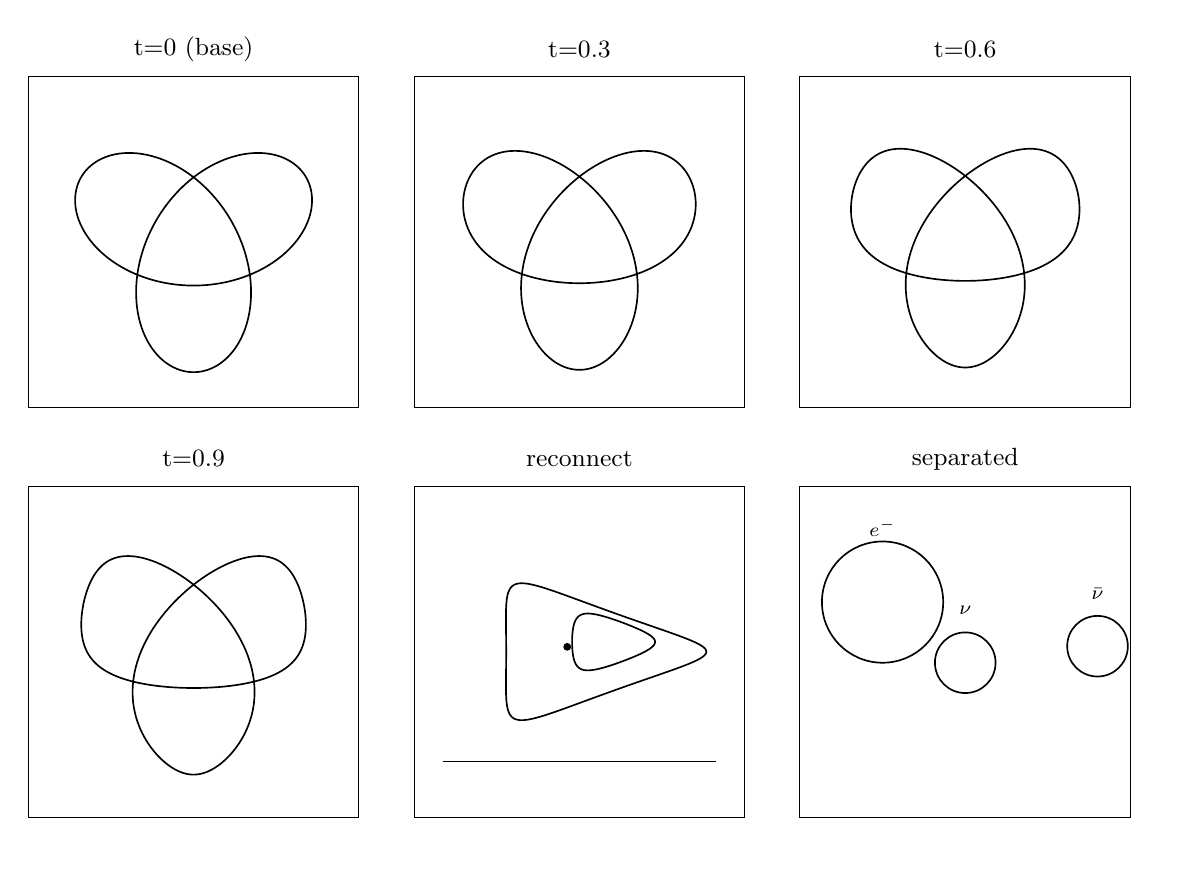
\begin{tikzpicture}[x=1cm,y=1cm]

    % ----------------------------
    % Layout parameters (in cm)
    % ----------------------------
    \pgfmathsetmacro{\W}{4.2}
    \pgfmathsetmacro{\H}{4.2}
    \pgfmathsetmacro{\Xgap}{0.7}
    \pgfmathsetmacro{\Ygap}{1.0}
    \pgfmathsetmacro{\Whalf}{\W/2}
    \pgfmathsetmacro{\Hhalf}{\H/2}

    \pgfmathsetmacro{\xA}{0}
    \pgfmathsetmacro{\xB}{\W+\Xgap}
    \pgfmathsetmacro{\xC}{2*(\W+\Xgap)}
    \pgfmathsetmacro{\yTop}{\H+\Ygap}
    \pgfmathsetmacro{\yBot}{0}

    % ----------------------------
    % Trefoil projection with perturbation amplitude eps
    % x(t) = sin t + 2 sin 2t + eps sin 5t
    % y(t) = cos t - 2 cos 2t + eps cos 4t
    % (TikZ trig uses degrees)
    % ----------------------------
     \newcommand{\TrefoilPerturbed}[1]{%
       % IMPORTANT: do not use \t as the plot variable (TeX accent macro).
       % Use an explicit pgfplots variable instead.
       \draw[line width=0.6pt]
         plot[domain=0:360,variable=\ang,samples=260,smooth]
           ({sin(\ang)+2*sin(2*\ang)+(#1)*sin(5*\ang)},
            {cos(\ang)-2*cos(2*\ang)+(#1)*cos(4*\ang)});
     }

    % ----------------------------
    % Panel templates
    % ----------------------------
    \newcommand{\PanelFrame}[3]{% shiftx, shifty, title
      \begin{scope}[shift={(#1,#2)}]
        \draw[black] (0,0) rectangle (\W,\H);
        \node[font=\small] at (\Whalf,\H+0.35) {#3};
      \end{scope}
    }

    \newcommand{\PanelTrefoil}[4]{% shiftx, shifty, title, eps
      \PanelFrame{#1}{#2}{#3}
      \begin{scope}[shift={(#1,#2)}]
        \begin{scope}[shift={(\Whalf,\Hhalf)},scale=0.55]
          \clip (-3.55,-3.55) rectangle (3.55,3.55);
          \TrefoilPerturbed{#4}
        \end{scope}
      \end{scope}
    }

% ----------------------------
% Panel: reconnection-like schematic (bounded + clipped)  [USES YOUR \W,\H,\Whalf,\Hhalf]
% ----------------------------
    \newcommand{\PanelReconnect}[3]{% shiftx, shifty, title
        \PanelFrame{#1}{#2}{#3}
        \begin{scope}[shift={(#1,#2)}]
        % Clip strictly to the panel interior
        \clip (0.05,0.05) rectangle (\W-0.05,\H-0.05);

        % Draw centered content
        \begin{scope}[shift={(\Whalf,\Hhalf)},scale=0.62]

        % Compact outer loop (always inside bounds at this scale)
        \draw[line width=0.6pt]
        plot[domain=0:360,variable=\ang,samples=240,smooth]
        ({ 2.05*cos(\ang) + 0.55*cos(2*\ang) },
            { 1.25*sin(\ang) - 0.35*sin(2*\ang) });

        % Small inner loop (neck/surgery cue)
        \draw[line width=0.6pt]
        plot[domain=0:360,variable=\ang,samples=220,smooth]
        ({ 0.85*cos(\ang) + 0.15*cos(2*\ang) + 0.55 },
            { 0.55*sin(\ang) - 0.10*sin(2*\ang) + 0.20 });

        % Reconnection marker
        \fill (-0.25,0.10) circle (0.08);

        % Reference line (kept inside)
        \draw[line width=0.6pt] (-2.8,-2.25) -- (2.8,-2.25);

        \end{scope}
        \end{scope}
    }

% ----------------------------
% Panel: separated components (bounded + clipped)  [USES YOUR \W,\H,\Whalf,\Hhalf]
% ----------------------------
    \newcommand{\PanelSeparated}[3]{% shiftx, shifty, title
        \PanelFrame{#1}{#2}{#3}
        \begin{scope}[shift={(#1,#2)}]
            \begin{scope}[shift={(\Whalf,\Hhalf)},scale=0.70]
                \clip (-3.55,-3.55) rectangle (3.55,3.55);

                % --- Three separated loop components (schematic) ---
                % Left: larger loop (label as e-)
                \draw[line width=0.6pt](-1.5, 0.9) circle [radius=1.10];
                \node[font=\scriptsize] at (-1.5, 2.25) {$e^{-}$};

                % Center: small loop (label as nu)
                \draw[line width=0.6pt](0.0,-0.2) circle [radius=0.55];
                \node[font=\scriptsize] at (0.0, 0.75) {$\nu$};

                % Right: small loop (label as anti-nu)
                \draw[line width=0.6pt](2.4, 0.1) circle [radius=0.55];
                \node[font=\scriptsize] at (2.4, 1.05) {$\bar{\nu}$};
            \end{scope}
        \end{scope}
    }



    % ----------------------------
    % 2x3 panel placement
    % ----------------------------
    % Top row: increasing perturbation
    \PanelTrefoil{\xA}{\yTop}{t=0 (base)}{0.00}
    \PanelTrefoil{\xB}{\yTop}{t=0.3}{0.054}  % 0.18*0.3
    \PanelTrefoil{\xC}{\yTop}{t=0.6}{0.108}  % 0.18*0.6

    % Bottom row: stronger perturbation + schematic decay panels
    \PanelTrefoil{\xA}{\yBot}{t=0.9}{0.162}  % 0.18*0.9
    \PanelReconnect{\xB}{\yBot}{reconnect}
    \PanelSeparated{\xC}{\yBot}{separated}

    \end{tikzpicture}

    \caption{Schematic swirl-knot evolution under perturbation and reconnection-like decay (illustrative placeholder). Top row: trefoil-like curve under increasing perturbation amplitude. Bottom row: a reconnection-like transition and separated components. Replace the last two panels with SST evolution output once the perturbation + reconnection/decay rule is fixed.}
    \label{fig:knot-evolution-panel}
    \end{figure}



\section{Refined $\Xi(K)$ Functional (parametric analytic form)}
\label{sec:v076-xi}

For a knot or link configuration $K$ (possibly multi-component), define the geometric primitives:
arc-length $s$, curvature $\kappa(s)$, torsion $\tau(s)$, and (for multi-component links) pairwise
linking numbers $\mathrm{Lk}_{ij}$. Introduce a core-scale radius $a$ (e.g.\ proportional to $r_c$)
and ropelength
\begin{equation}
\mathcal{R}(K)=\frac{L(K)}{a},
\qquad
L(K)=\int_K ds.
\end{equation}

We define a \emph{dimensionless} effective energy functional
\begin{equation}
\Xi(K)=\lambda_L\,\mathcal{R}(K)
\;+\;\lambda_\kappa \int_K \big(a\,\kappa(s)\big)^2 \,\frac{ds}{a}
\;+\;\lambda_\tau \int_K \big(a\,\tau(s)\big)^2 \,\frac{ds}{a}
\;+\;\lambda_{\rm link}\sum_{i<j}\big|\mathrm{Lk}_{ij}\big|
\;+\;\lambda_{\rm hel}\,\big|\mathcal{H}(K)\big|,
\label{eq:XiK}
\end{equation}
where $\mathcal{H}(K)$ denotes a helicity/Hopf-type topological charge for the configuration (in the
single-component case, this may be represented via twist+writhe proxies once a ribbon framing is chosen).
The coefficients $\{\lambda_L,\lambda_\kappa,\lambda_\tau,\lambda_{\rm link},\lambda_{\rm hel}\}$ are
dimensionless EFT parameters.

\paragraph{Interpretation.}
The $\lambda_L$ term captures a line-tension contribution (length/ropelength). The curvature and torsion terms
penalize bending and chirality. The linking term encodes multi-component coupling constraints. The helicity term
captures global topological stabilization/selection. The v0.7.6 deliverable is to (i) state \eqref{eq:XiK} explicitly,
and (ii) report best-fit / constrained coefficient sets (even if only for the lepton and nucleon anchor classes).


\section{Gauge Sector: $\mathrm{U}(1)$ Field Strength from Helicoidal Excitations}
\label{sec:v076-u1}

We outline a minimal EFT derivation of a Maxwell-type $\mathrm{U}(1)$ sector from helicoidal excitations of the
swirl flow. Consider small, divergence-free perturbations $\delta\mathbf{v}(x,t)$ about a background configuration,
with $\nabla\cdot\delta\mathbf{v}=0$. Introduce a vector potential $\mathbf{A}$ and scalar potential $\Phi$ via the
identification
\begin{equation}
\delta\mathbf{v} \equiv \frac{1}{\Lambda}\,\mathbf{A},
\qquad
\delta p \equiv \frac{1}{\Lambda}\,\Phi,
\end{equation}
where $\Lambda$ is a constant with units such that $\mathbf{A}$ carries the usual electromagnetic dimensions in the
effective theory (to be fixed by matching).

Define the effective fields
\begin{equation}
\mathbf{E} \equiv -\partial_t \mathbf{A}-\nabla\Phi,
\qquad
\mathbf{B} \equiv \nabla\times\mathbf{A}.
\end{equation}
The most general quadratic, parity-even, gauge-invariant local action for these fields is
\begin{equation}
\mathcal{L}_{\mathrm{U}(1)}=\frac{1}{2\mu_0}\left(\frac{1}{c_{\rm hel}^2}\,\mathbf{E}^2-\mathbf{B}^2\right)
\;=\;-\frac{1}{4\mu_0}\,F_{\mu\nu}F^{\mu\nu},
\label{eq:MaxwellEFT}
\end{equation}
where $F_{\mu\nu}=\partial_\mu A_\nu-\partial_\nu A_\mu$ and $c_{\rm hel}$ is the propagation speed of the helicoidal
mode. Matching to the flow kinetic energy density,
\begin{equation}
\frac{1}{2}\rho_{\!f}\,|\delta\mathbf{v}|^2 = \frac{1}{2}\rho_{\!f}\,\frac{1}{\Lambda^2}\,|\mathbf{A}|^2,
\end{equation}
fixes $\mu_0$ and $\Lambda$ (or equivalently $\epsilon_0$) once the normalization convention for $A_\mu$ is selected.
In v0.7.6, the key goal is to provide (i) the identification map, and (ii) a consistency check that the radiative mode
described by \eqref{eq:MaxwellEFT} is compatible with the underlying swirl-flow linear response about a chosen background.

\paragraph{Deliverable.}
Provide a concrete background configuration and show that the linearized equations admit a helicoidal propagating solution
whose quadratic action reduces to \eqref{eq:MaxwellEFT} with a well-defined $c_{\rm hel}$.


\section{Glossary}
\label{sec:v076-glossary}

\begin{description}
\item[swirl string] A stable, localized excitation in the incompressible medium supporting quantized circulation and topological class labels.
\item[scalar clock field $\chi$] Scalar foliation/clock degree of freedom sourcing far-field momentum flux; in the minimal gravity sector obeys a Poisson-type closure.
\item[Swirl Clock $S_t^{\boldsymbol{\circlearrowleft}}$] Dimensionless local time-scaling indicator tied to tangential swirl speed and rotational state (matter orientation).
\item[effective fluid density $\rho_{\!f}$] Coarse-grained density scale used in macroscopic energy/momentum densities.
\item[swirl energy density $\rho_{\!E}$] Energy density associated with swirl motion; often used to define $\rho_{\!m}=\rho_{\!E}/c^2$.
\item[mass-equivalent density $\rho_{\!m}$] Effective mass density defined from swirl energy density via $c^2$ conversion.
\item[core radius $r_c$] Canonical microscopic length scale setting core/filament radius and coarse-graining cutoffs.
\item[characteristic swirl speed $\mathbf{v}_{\!\boldsymbol{\circlearrowleft}}$] Canonical tangential swirl speed scale used in SST benchmarks.
\item[velocity field $\mathbf{v}$] Incompressible flow velocity of the effective medium; $\nabla\cdot\mathbf{v}=0$.
\item[vorticity $\boldsymbol{\omega}$] Curl of velocity, $\boldsymbol{\omega}=\nabla\times\mathbf{v}$.
\item[circulation $\Gamma$] Line integral of velocity around a loop, $\Gamma=\oint \mathbf{v}\cdot d\boldsymbol{\ell}$.
\item[pressure well] A region of reduced effective pressure associated with sustained swirl motion, generating attraction toward the minimum.
\item[irrotational envelope] Outer region with $\nabla\times\mathbf{v}\approx 0$ that mediates far-field interactions.
\item[ropelength $\mathcal{R}$] Dimensionless length $\mathcal{R}=L/a$ for a curve with core radius $a$.
\item[curvature $\kappa$] Local bending rate of an embedded curve; enters bending-energy penalties.
\item[torsion $\tau$] Local chirality/twisting rate of an embedded curve; enters chirality-energy penalties.
\item[linking number $\mathrm{Lk}$] Integer topological invariant counting linkings between components of a link.
\item[writhe $\mathrm{Wr}$] Geometric measure of coiling of a curve; depends on embedding.
\item[twist $\mathrm{Tw}$] Framing-dependent twist of a ribbon; with writhe gives linking via $\mathrm{Lk}=\mathrm{Tw}+\mathrm{Wr}$.
\item[helicity $\mathcal{H}$] Integral topological measure of linkage/coiling of field lines; conserved in ideal settings.
\item[Hopf charge] Integer (or quantized) invariant characterizing linked preimages in map-based descriptions; used as a stability proxy.
\item[Kelvin mode] Small oscillation mode of a filament/loop; quantization or suppression of these modes controls orbital spectra in SST.
\item[director field] Internal orientation field (e.g.\ $U(2)$ or $U(3)$ valued) encoding internal degrees of freedom.
\item[multi-director sector] Set of coupled director fields whose low-energy modes reproduce effective gauge symmetries.
\item[helicoidal excitation] Propagating, screw-like perturbation mode (phase + rotation) used as the candidate $\mathrm{U}(1)$ radiative mode.
\end{description}

\clearpage

    
    \appendix

% ======================================================================
    \section{Fundamental Hydrodynamic Constants (Zero-Parameter Triplet)}
    \label{app:constants_triplet}
% ======================================================================

Canon v0.7.6 reinstates the \emph{primitive constant triplet}
\begin{equation}
    (\Gamma_0,\ \rho_{\!f},\ r_c),
\end{equation}
as the minimal generating set for the emergent sector.
The circulation quantum is defined by the canonical swirl speed scale
$\lVert \mathbf{v}_{\!\boldsymbol{\circlearrowleft}}\rVert$ via
\begin{equation}
    \Gamma_0 \equiv 2\pi r_c\,\lVert \mathbf{v}_{\!\boldsymbol{\circlearrowleft}}\rVert,
\end{equation}
while $\rho_{\!f}$ fixes the inertial scale of the background condensate and $r_c$
fixes the ultraviolet core regularization.

\paragraph{Derived quantities.}
With $(\Gamma_0,\rho_{\!f},r_c)$ fixed, the Canon treats the following as derived:
\begin{itemize}
    \item stiffness/mass scale in the clock EFT (encoded by $\mu_\tau$);
    \item long-range coupling $G_{\rm eff}$ (Poisson limit);
    \item swirl-electromagnetic conversion scales ($\kappa_A$ in
    Eq.~\eqref{eq:AB_from_vperp});
    \item knot energies and masses via the core density sector
    (Section~\ref{sec:mass_expanded}).
\end{itemize}

% ======================================================================
    \section{Hydrodynamic Energy--Momentum Tensor and Momentum Conservation}
    \label{app:stress_tensor}
% ======================================================================

For an inviscid condensate with mass density $\rho$ and velocity $\mathbf{v}$,
the standard (nonrelativistic) momentum-flux tensor is
\begin{equation}
    T_{ij} = \rho\,v_i v_j + p\,\delta_{ij},
    \label{eq:stress_tensor_basic}
\end{equation}
where $p$ is the pressure enforcing incompressibility and $\delta_{ij}$ is the
Kronecker delta. Local momentum conservation takes the form
\begin{equation}
    \partial_t(\rho v_i) + \partial_j T_{ij} = 0,
\end{equation}
which is equivalent to the Euler equations when $\rho$ is constant.

\paragraph{Covariant packaging (module level).}
In SST, the clock/foliation potential $\chi$ and its EFT completion introduce an
additional scalar stress contribution. Canon v0.7.6 records this schematically as
\begin{equation}
    T_{\mu\nu}^{\rm (tot)} \;=\; T_{\mu\nu}^{\rm (fluid)} \;+\; T_{\mu\nu}^{(\chi)},
    \qquad
    \nabla_\mu T^{\mu}{}_{\nu}{}^{\rm (tot)}=0,
\end{equation}
where $T_{\mu\nu}^{(\chi)}$ is computed from the quadratic clock action in the usual
field-theoretic way. This provides the direct route for writing SST dynamics in a
form comparable to GR conservation statements, while remaining anchored in
hydrodynamic variables.


% =====================================================================
\section{Numerical Benchmarks and Reproducibility}
\label{app:benchmarks}

This Canon is accompanied by a minimal, reproducible numerical evaluation of the invariant mass kernel (Sec.~\ref{sec:mass_kernel}) and the binding-corrected atomic/molecular aggregation model (Sec.~\ref{sec:mass_chemistry}). The reference implementation is the script \texttt{SST\_INVARIANT\_MASS.py} (user-space), which produces CSV artifacts that can be cited, archived, and re-generated.

\paragraph{Canonical outputs (CSV artifacts).}
The numerical engine emits the following machine-readable tables:
\begin{itemize}
    \item \texttt{SST\_Invariant\_Mass\_Results\_exact\_closure.csv} --- full table of particle, atomic, and selected molecular masses in the \emph{exact\_closure} calibration mode.
    \item \texttt{SST\_Invariant\_Mass\_Results\_all\_modes.csv} --- the same table augmented with \emph{canonical} and \emph{sector\_norm} mode columns for cross-mode comparison.
    \item \texttt{SST\_Atom\_Toy\_Masses.csv} --- a reduced ``toy'' subset used for rapid regression tests.
\end{itemize}

\paragraph{Input requirements for numerical reproduction.}
A faithful re-run requires only:
(i) the Canon constants \((\rho_{\!f}, \rho_{\text{core}}, r_c, \lVert \mathbf{v}_{\!\boldsymbol{\circlearrowleft}}\rVert)\),
(ii) the particle topology assignments \((k,g,n)\) and the mode-dependent ropelength proxies \(L_{\text{tot}}(T)\),
and (iii) a binding-energy model to convert ``sum-of-parts'' nucleon masses into nuclear masses (here: a SEMF proxy; Sec.~\ref{sec:mass_chemistry}).

\paragraph{Benchmark summary (exact\_closure mode).}
For the provided run artifacts, the element-level accuracy after binding correction is at the \(\mathcal{O}(10^{-2})\) relative-error level across the periodic table (excluding chemical binding and isotopic fine structure), while certain large molecules are outside scope (chemical bonding, electron correlations, and non-additive geometry are not modeled). A compact summary is given in Table~\ref{tab:benchmarks_summary}.

\begin{table}[t]
\centering
\caption{Empirical error summary for the provided CSV artifact \texttt{SST\_Invariant\_Mass\_Results\_exact\_closure.csv}. ``Mean abs.'' denotes the mean absolute relative error, and ``P95 abs.'' denotes the 95th percentile of the absolute relative error.}
\label{tab:benchmarks_summary}
\begin{tabular}{lrrrr}
\toprule
Class & Count & Mean abs.\ (\%) & P95 abs.\ (\%) & Max abs.\ (\%) \\
\midrule
Particles (e,p,n) & 3 & 0.000 & 0.000 & 0.000 \\
Elements (Z=1--92) & 92 & 0.846 & 0.911 & 2.608 \\
Molecules (selected) & 18 & 4.780 & 1.202 & 79.036 \\
\bottomrule
\end{tabular}
\end{table}

\paragraph{Interpretation and scope.}
The molecule outlier (\texttt{C8H10N4O2}, caffeine) highlights a limitation of additive ``sum-of-atoms'' assembly when the model lacks explicit chemical binding, electronic structure, and non-additive geometry. In contrast, the \(\lesssim 1\%\) typical elemental accuracy suggests that (i) baryon-sector closure and (ii) the binding-energy proxy are numerically consistent at the level of bulk nuclear systematics. Canon-conform upgrades that improve numerical fidelity without changing the invariant kernel include:
\begin{enumerate}
    \item replacing SEMF coefficients by a Canon-derived interaction functional (or by a table-driven correction from measured nuclear binding energies),
    \item extending the molecular model to include an explicit chemical binding correction at the eV scale (with isotopic bookkeeping),
    \item replacing the ropelength proxies by a knot-geometry library \(L(K)\) derived from numerical minimizers (e.g.\ tube-energy minimization), and
    \item adding uncertainty propagation (Monte Carlo) for \(\rho_{\text{core}}, r_c,\lVert \mathbf{v}_{\!\boldsymbol{\circlearrowleft}}\rVert\) and any fitted geometric factors.
\end{enumerate}

% =====================================================================
    \section{Reference Constants}
    \begin{itemize}
        \item $\mathbf{v}_{\circlearrowleft} = 1.09384563 \times 10^6$ m s$^{-1}$
        \item $r_c = 1.40897017 \times 10^{-15}$ m
        \item $\rhocore = 3.893435827 \times 10^{18}$ kg m$^{-3}$
        \item $F_{\text{swirl}}^{\max} = 29.053507$ N
    \end{itemize}



\section{Integrated Response to Critical Inquiry}

\noindent \textbf{Subject:} Addressing the Synthesis of SST Canon v0.7.6 and the Relational TOA Framework \\
\textbf{Context:} Response to peer-inquiry regarding conservation robustness, scale dependence, and experimental falsifiability of the unified Clock-Gravity sector.

\subsection*{1. On Conservation Robustness in Open Quantum Systems}
\noindent \textbf{Critique:} \textit{In realistic quantum systems involving creation and annihilation, is the event current conservation $\nabla_\mu j^\mu_{ev} = 0$ robust? Does SST predict clock drifts?}

\noindent \textbf{SST Response:}
In Swirl-String Theory, particle "creation" and "annihilation" are topological reconnection events, not disappearances into nothingness. By Stokes' Theorem, the total vorticity flux is conserved across a reconnection singularity.
\begin{itemize}
    \item \textbf{Topological Continuity:} An annihilation event ($e^+ + e^- \to \gamma\gamma$) transforms the event current from a mass-knot topology (particle-like) to a shear-wave topology (photon-like), but the underlying hydrodynamic current remains conserved.
    \item \textbf{Predicted Anomaly:} We predict a specific "clock drift" in high-energy scattering. In regions of intense reconnection density, the local event count $N$ fluctuates relative to the background vacuum rate. This manifests as an \textit{anomalous decoherence rate} in the Time-of-Arrival distribution for short-lived resonances, deviating from the standard Breit-Wigner width by a factor proportional to the local swirl variance $\sigma_\tau^2$.
\end{itemize}

\subsection*{2. On the Coarse-Graining Scale $\ell$}
\noindent \textbf{Critique:} \textit{Does the coarse-graining scale $\ell$ act as a new hidden constant, effectively reintroducing a preferred frame?}

\noindent \textbf{SST Response:}
The scale $\ell$ is not an external parameter but an \textbf{emergent correlation length}, analogous to the Debye length in plasmas or the phononic mean free path in superfluids.
\begin{itemize}
    \item \textbf{Dynamic Scale:} In the vacuum ground state, $\ell \approx r_c$ (the core radius). However, in the presence of matter, $\ell$ adapts to the local vortex density.
    \item \textbf{Relationality:} The theory remains relational because $\ell$ is defined by the clock field itself. High-frequency clocks (probing small $\ell$) perceive a "grainy" time, while low-frequency clocks (averaging over large $\ell$) perceive a smooth continuum. The "preferred foliation" is locally defined by the fluid's vorticity vector $u^\mu$, which preserves general covariance in the continuum limit.
\end{itemize}

\subsection*{3. On the "Massive Clock Sector" and Gravity Duality}\label{sec:massive-clock-gravity}
\noindent \textbf{Critique:} \textit{Does the massive clock parameter $\mu_\tau$ imply a new scalar field? Is the TOA field $T(x)$ identical to the SST gravity field $\chi(x)$?}

\noindent \textbf{SST Response:}
\textbf{Yes, they are identical.} This constitutes the central unification of Canon v0.7.6.
\begin{itemize}
    \item \textbf{The Identification:} The "Clock Field" $T(x)$ in the TOA formalism is the potential of the flow, while the "Gravity Field" $\chi(x)$ is the logarithmic rate of that flow ($S_\circ$). They are related by the stiffness of the vacuum:
    \begin{equation}
        \chi(x) \propto \mu_\tau^2 \, T(x)
    \end{equation}
    \item \textbf{Physical Meaning:} The "mass" $\mu_\tau$ corresponds to the vacuum's bulk modulus (resistance to compression). Gravity is the long-range relaxation of this stiff field.
    \item \textbf{Redshift as Variance:} Gravitational redshift is reinterpreted as a signal-to-noise effect. In a deep potential well (dense $\chi$), the event density is higher, but the clock variance $\sigma_\tau^2$ increases due to vortex crowding. Time "slows down" because the information content (signal) per unit of noise decreases.
\end{itemize}

\subsection*{4. On Experimental Falsifiability ($\sigma_\tau$)}
\noindent \textbf{Critique:} \textit{Can the predicted clock-induced variance be isolated from standard environmental decoherence?}

\noindent \textbf{SST Response:}
The "Intrinsic Clock Noise" $\sigma_\tau$ possesses a unique spectral signature distinct from thermal ($k_B T$) or $1/f$ noise.
\begin{itemize}
    \item \textbf{Shot Noise Signature:} SST Clock Noise is driven by discrete topological knot crossings. It exhibits Poissonian shot-noise statistics peaking at the Zitterbewegung frequency ($\sim 10^{21}$ Hz).
    \item \textbf{Proposed Experiment:} We propose an interferometric test with \textbf{entangled atomic clocks} at zero spatial separation but differing gravitational potentials (or simulated swirl potentials). Standard decoherence scales with path separation; SST clock noise scales with the \textit{potential difference} even at zero path difference. A non-vanishing variance in this configuration would falsify standard QM in favor of SST.
\end{itemize}

\subsection*{5. On the Unification of Currents}
\noindent \textbf{Critique:} \textit{Is the distinction between the Event Current $J^\mu$ (Canon) and the Flux $j^\mu$ (TOA) redundant?}

\noindent \textbf{SST Response:}
They are dual representations of the same underlying conservation law.
\begin{itemize}
    \item $J^\mu$ represents the \textbf{Source} (the location of the knots/matter).
    \item $j^\mu$ represents the \textbf{Probe} (the flow through the detector).
    \item \textbf{Unified Origin:} In the full Lagrangian (Canon Eq. 12), both arise from the Noether current associated with the $U(1)$ phase symmetry of the condensate wavefunction $\psi = \sqrt{\rho} e^{i\theta}$:
    \begin{equation}
        J_{\text{total}}^\mu = \rho_f (\partial^\mu \theta - W^\mu)
    \end{equation}
    This confirms that the apparent duplication is merely a functional distinction between "system" and "apparatus" in the measurement setup, which vanishes in the holistic fluid description.
\end{itemize}

    \section*{Appendix X: Velocity-Dependent Mass Functional and Preferred-Frame Corrections}
    \addcontentsline{toc}{section}{Appendix X: Velocity-Dependent Mass Functional and Preferred-Frame Corrections}

    \subsection*{X.1 Scope and purpose}

        This appendix supplements Theorem~\ref{thm:EM_no_gravity} by making explicit
        how preferred-frame effects arise from velocity-dependent sampling of the
        SST mass functional.

        This appendix fixes the canonical interpretation of preferred-frame effects in
        Swirl-String Theory (SST). It establishes that such effects arise from
        \emph{velocity-dependent corrections to the mass functional} and do not correspond
        to additional forces, interactions, or violations of energy conservation.

        The purpose of this appendix is definitional. No new dynamical assumptions are
        introduced.

    \subsection*{X.2 Mass functional in SST}

        In SST, inertial and gravitational mass are not primitive quantities.
        They are defined through an integral over the local swirl energy density,
        \begin{equation}
            M \;=\; \mathcal{C} \int_V \rho_{\!E}(\mathbf{x}) \, dV ,
        \end{equation}
        where $\rho_{\!E}$ denotes the local swirl energy density and $\mathcal{C}$ is a
        fixed normalization constant determined by the SST mass calibration
        (see SST-59).

        The evaluation of $\rho_{\!E}$ is implicitly referenced to a local clock and
        foliation structure. In covariant formulations this structure is represented
        by a unit timelike vector field $u^\mu$ satisfying
        \begin{equation}
            u^\mu u_\mu = -1 ,
        \end{equation}
        which defines the local notions of rest, simultaneity, and proper time.

    \subsection*{X.3 Boosted observers and effective mass}

        Consider an observer or laboratory moving with spatial velocity $\mathbf{v}$
        relative to the foliation defined by $u^\mu$.
        Such an observer samples the same physical configuration through a
        \emph{boosted slicing} of the clock field.

        As a consequence, the effective energy density entering the mass functional
        is modified. The resulting effective mass is therefore velocity dependent,
        \begin{equation}
            M_{\mathrm{eff}}(\mathbf{v})
            \;=\;
            \mathcal{C}
            \int_V
            \rho_{\!E}\!\left(u^\mu + \delta u^\mu(\mathbf{v})\right)
            \, dV .
        \end{equation}

        This dependence is purely kinematical and reflects how the energy density is
        sampled by the moving observer.

    \subsection*{X.4 Velocity expansion of the mass functional}

        For velocities small compared to the characteristic signal speed $c$,
        the effective mass admits a systematic expansion in powers of $v/c$.
        To second order,
        \begin{equation}
            M_{\mathrm{eff}}(\mathbf{v})
            =
            M_0
            \left[
                1
                + \beta_1 \, \frac{\mathbf{v}\!\cdot\!\hat{u}}{c}
                + \beta_2 \, \frac{(\mathbf{v}\!\cdot\!\hat{u})^2}{c^2}
                + \mathcal{O}\!\left(\frac{v^3}{c^3}\right)
            \right],
        \end{equation}
        where:
        \begin{itemize}
            \item $M_0$ is the mass evaluated in the foliation rest frame,
            \item $\hat{u}$ denotes the spatial direction selected by the clock field,
            \item $\beta_1$ and $\beta_2$ are dimensionless coefficients fixed by the SST
            dynamics.
        \end{itemize}

        The expansion expresses a direction-dependent redistribution within the mass
        functional and does not imply the presence of new interaction terms.

    \subsection*{X.5 Relation to PPN preferred-frame parameters}

        In the weak-field, low-velocity regime, the coefficients $\beta_1$ and $\beta_2$
        map directly onto the standard Parameterized Post-Newtonian preferred-frame
        parameters,
        \begin{equation}
            \beta_1 \;\leftrightarrow\; \alpha_1,
            \qquad
            \beta_2 \;\leftrightarrow\; \alpha_2 .
        \end{equation}

        Accordingly:
        \begin{itemize}
            \item $\alpha_1$ characterizes the linear velocity dependence of the SST mass
            functional,
            \item $\alpha_2$ characterizes the quadratic, anisotropic velocity dependence.
        \end{itemize}

        Within SST, preferred-frame parameters therefore quantify corrections to the
        \emph{definition of mass}, rather than modifications of the gravitational
        force law.

    \subsection*{X.6 Interpretation and limiting cases}

        The canonical interpretation fixed here implies:
        \begin{enumerate}
            \item Preferred-frame effects in SST do not introduce additional long-range
            forces.
            \item Energy conservation is preserved; the corrections arise from internal
            redistribution within the mass functional.
            \item Suppression by powers of $v/c$ explains the small magnitude of
            preferred-frame signals and the dominance of astrophysical bounds.
        \end{enumerate}

        In the limit $\beta_1 = \beta_2 = 0$, the SST mass functional becomes
        velocity independent, reproducing the effective equivalence of inertial and
        gravitational mass assumed in General Relativity.

    \subsection*{X.7 Canonical status}

        The identification of preferred-frame parameters with coefficients in the
        velocity expansion of the SST mass functional is \emph{canonical}.
        Any experimental constraint on $\alpha_1$ or $\alpha_2$ therefore constrains
        the admissible form of the SST mass definition itself, not an auxiliary or
        additive interaction sector.


        
%================================================
% References
%================================================

\bibliographystyle{unsrt}
\begin{thebibliography}{99}

    \bibliography{canon_swirl_string_theory}
    \bibitem{ThurstonNotes}
    W.~P.~Thurston,
    \newblock \emph{The Geometry and Topology of Three-Manifolds},
    \newblock Princeton Univ. Lecture Notes, 1979.

    \bibitem{NeumannZagier1985}
    W.~D.~Neumann and D.~Zagier,
    \newblock Volumes of hyperbolic three-manifolds,
    \newblock \emph{Topology} \textbf{24}(3):307--332, 1985. \url{https://doi.org/10.1016/0040-9383(85)90003-4}

    \bibitem{AdamsWeeks1992}
    C.~Adams, M.~Hildebrand, and J.~Weeks,
    \newblock Hyperbolic invariants of knots and links,
    \newblock \emph{Trans. Amer. Math. Soc.} \textbf{326}(1):1--56, 1992.

    \bibitem{Lewin1981}
    L.~Lewin,
    \newblock \emph{Polylogarithms and Associated Functions},
    \newblock North-Holland, 1981.

    \bibitem{KAtlas52}
    D.~Bar-Natan et al.,
    \newblock The Knot Atlas: entry \(5_2\),
    \newblock \url{https://katlas.org/wiki/5_2}.

    \bibitem{KAtlas61}
    D.~Bar-Natan et al.,
    \newblock The Knot Atlas: entry \(6_1\),
    \newblock \url{https://katlas.org/wiki/6_1}.

    \bibitem{Annala2025} T. Annala \emph{et al.}, ``Topologically protected vortex knots and links,'' \emph{Phys. Rev. Lett.}, 2025.
    \bibitem{Kleckner2016} D. Kleckner, L. Kauffman, W. Irvine, ``How superfluid vortex knots untie,'' \emph{Nat. Phys.} 12, 650–655 (2016).
    \bibitem{Ricca1996} R. Ricca, ``Applications of knot theory in fluid mechanics,'' \emph{Banach Center Publications}, Vol. 42 (1996).
    \bibitem{Purcell2025} D. Ibarra, D. Mathews, J. Purcell, ``On geometric triangulations of double twist knots,'' arXiv:2504.09901 (2025).
    \bibitem{Petersen2024} I. Petersen, A. Tsvietkova, ``Geometric structures and PSL$_2(\mathbb{C})$ representations of knot groups,'' \emph{Trans. AMS} (2024).


    \bibitem{SSTCanon05}
    Iskandarani, O.\ (2025).
    \emph{Swirl–String Theory Canon v0.5.8}.
    Internal manuscript (Canon).

    \bibitem{Rosetta05}
    Iskandarani, O.\ (2025).
    \emph{VAM–SST Rosetta v0.5}.
    Internal manuscript (Rosetta).

    \bibitem{IskandaraniTriad2025}
    O.~Iskandarani,
    ``The Hydrodynamic Triad: Unifying Gravity, Electromagnetism, and Quantum Mass
    via a Circulation-Based Vacuum Canon,''
    Zenodo (2025), DOI: 10.5281/zenodo.17728292.

    \bibitem{LandauLifshitzFM1987}
    Landau, L. D., \& Lifshitz, E. M.\ (1987).
    \emph{Fluid Mechanics} (2nd ed.). Pergamon.
    (Foundations of inviscid linearization and Bernoulli used in \eqref{eq:B5}.)

    \bibitem{MorseIngard1968}
    Morse, P. M., \& Ingard, K. U.\ (1968).
    \emph{Theoretical Acoustics}. Princeton University Press.
    (Standard monopole source \eqref{eq:B2} and far-field law \eqref{eq:B3}–\eqref{eq:B4}.)

    \bibitem{Pierce1989}
    Pierce, A. D.\ (1989/1991).
    \emph{Acoustics: An Introduction to Its Physical Principles and Applications} (2nd ed.). ASA.
    (Alternative derivations for \eqref{eq:B3}–\eqref{eq:B4}.)

    \bibitem{Westervelt1963}
    Westervelt, P. J.\ (1963).
    Parametric acoustic array.
    \emph{J. Acoust. Soc. Am.}, 35(4), 535–537.
    (Constitutive parametric pumping basis compatible with BASC inside $T$.)

    \bibitem{HamiltonBlackstock1998}
    Hamilton, M. F., \& Blackstock, D. T.\ (1998).
    \emph{Nonlinear Acoustics}. Academic Press.
    (Background on quadratic transduction and difference-frequency generation.)


    \bibitem{Einstein1905}
    A.~Einstein,
    \newblock Zur Elektrodynamik bewegter K{\"o}rper,
    \newblock {\em Annalen der Physik} \textbf{322}(10) (1905) 891--921.
    \newblock doi:10.1002/andp.19053221004.

    \bibitem{Minkowski1909}
    H.~Minkowski,
    \newblock Raum und Zeit,
    \newblock {\em Jahresbericht der Deutschen Mathematiker-Vereinigung} \textbf{18} (1909) 75--88.

    \bibitem{LevyLeblond1976}
    J.-M.~L{\'e}vy-Leblond,
    \newblock One more derivation of the Lorentz transformation,
    \newblock {\em American Journal of Physics} \textbf{44}(3) (1976) 271--277.
    \newblock doi:10.1119/1.10324.



    \bibitem{Batchelor1967}
    G.~K.~Batchelor, \emph{An Introduction to Fluid Dynamics} (Cambridge Univ. Press, 1967).
    \bibitem{Saffman1992}
    P.~G.~Saffman, \emph{Vortex Dynamics} (Cambridge Univ. Press, 1992).
    \bibitem{Onsager1949}
    L.~Onsager, ``Statistical Hydrodynamics,'' \emph{Nuovo Cimento} \textbf{6} (Suppl. 2), 279--287 (1949).
    \bibitem{Feynman1955}
    R.~P.~Feynman, ``Application of quantum mechanics to liquid helium,'' in \emph{Progress in Low Temperature Physics}, Vol.~1 (1955), pp.~17--53.

    \bibitem{Unruh1976}
    W.~G.~Unruh,
    ``Notes on black-hole evaporation,''
    \textit{Phys. Rev. D} \textbf{14}, 870--892 (1976).
    doi:10.1103/PhysRevD.14.870

    \bibitem{Crispino2008}
    L.~C.~B.~Crispino, A.~Higuchi, and G.~E.~A.~Matsas,
    ``The Unruh effect and its applications,''
    \textit{Rev. Mod. Phys.} \textbf{80}, 787--838 (2008).
    doi:10.1103/RevModPhys.80.787

    \bibitem{Barcelo2011}
    C.~Barcel\'o, S.~Liberati, and M.~Visser,
    ``Analogue gravity,''
    \textit{Living Rev. Relativ.} \textbf{14}, 3 (2011).
    doi:10.12942/lrr-2011-3

    \bibitem{KinslerAcoustics}
    L.~E.~Kinsler, A.~R.~Frey, A.~B.~Coppens, and J.~V.~Sanders,
    \textit{Fundamentals of Acoustics}, 4th ed.,
    Wiley, New York (2000).

    \bibitem{Deswal2025}
    A.~Deswal, N.~Arya, K.~Lochan, and S.~K.~Goyal,
    ``Time-Resolved and Superradiantly Amplified Unruh Effect,''
    \textit{Phys. Rev. Lett.} (2025), arXiv:2501.16219.

    \bibitem{GrossHaroche1982}
    M.~Gross and S.~Haroche,
    ``Superradiance: An essay on the theory of collective spontaneous emission,''
    \textit{Phys. Rep.} \textbf{93}, 301--396 (1982).
    doi:10.1016/0370-1573(82)90102-8

    \bibitem{Lochan2020}
    K.~Lochan, S.~Chakraborty, and T.~Padmanabhan,
    ``Detecting Acceleration-Enhanced Vacuum Fluctuations,''
    \textit{Phys. Rev. Lett.} \textbf{125}, 241301 (2020).
    doi:10.1103/PhysRevLett.125.241301

    \bibitem{WangBlencowe2021}
    H.~Wang and M.~P.~Blencowe,
    ``Coherently Amplifying Photon Production from Vacuum,''
    \textit{Commun. Phys.} \textbf{4}, 62 (2021).
    doi:10.1038/s42005-021-00576-9



    \bibitem{Zheng2025}
    H.~T.~Zheng, Y.~Zhou, Q.~Guo, and L.~Zhou,
    ``Enhancing Analog Unruh Effect via Superradiance,''
    \textit{Phys. Rev. Research} \textbf{7}, 013027 (2025).
    doi:10.1103/PhysRevResearch.7.013027

    \bibitem{Saha2025}
    S.~Saha, T.~Galley, and E.~Mart\'in-Mart\'inez,
    ``Emergence of Unruh Prethermalization in Many-Body Systems,''
    (2025), arXiv:2509.05816.

    \bibitem{Steinhauer2016}
    J.~Steinhauer,
    ``Observation of quantum Hawking radiation and its entanglement in an analogue black hole,''
    \textit{Nat. Phys.} \textbf{12}, 959--965 (2016).
    doi:10.1038/nphys3863

    \bibitem{Gooding2020}
    C.~Gooding, S.~Weinfurtner, and W.~G.~Unruh,
    ``Superradiant scattering from a hydrodynamic vortex,''
    \textit{Phys. Rev. D} \textbf{101}, 024050 (2020).
    doi:10.1103/PhysRevD.101.024050

    \bibitem{doCarmo-diff-geom-2016}
    M.~P.~do Carmo,
    \textit{Differential Geometry of Curves and Surfaces},
    revised and updated second edition,
    Dover Publications, Mineola, NY (2016).
% permalink: https://store.doverpublications.com/0486806995.html

    \bibitem{Ratcliffe-hyperbolic-2006}
    J.~G.~Ratcliffe,
    \textit{Foundations of Hyperbolic Manifolds}, 2nd ed.,
    Graduate Texts in Mathematics, Vol.~149,
    Springer, New York (2006).
    doi:10.1007/978-0-387-47322-5

    \bibitem{Thurston-3manifolds-1997}
    W.~P.~Thurston,
    \textit{Three-Dimensional Geometry and Topology, Vol.~1},
    Princeton Mathematical Series 35,
    Princeton University Press, Princeton, NJ (1997).
% permalink: https://press.princeton.edu/books/hardcover/9780691084219/three-dimensional-geometry-and-topology-volume-1

    \bibitem{Sornette1998}
    D.~Sornette,
    ``Discrete scale invariance and complex dimensions,''
    \emph{Physics Reports} \textbf{297}, 239--270 (1998).
    doi:10.1016/S0370-1573(97)00076-8.

    \bibitem{GluzmanSornette2002}
    S.~Gluzman and D.~Sornette,
    ``Log-periodic route to fractal functions,''
    \emph{Physical Review E} \textbf{65}, 036142 (2002).
    doi:10.1103/PhysRevE.65.036142.

    \bibitem{BaakeGrimm2013}
    M.~Baake and U.~Grimm,
    \emph{Aperiodic Order. Volume~1: A Mathematical Invitation},
    Encyclopedia of Mathematics and its Applications, Vol.~149
    (Cambridge University Press, Cambridge, 2013).
    doi:10.1017/CBO9781139025256.

    \bibitem{Moffatt1969}
    H.~K.~Moffatt,
    ``The degree of knottedness of tangled vortex lines,''
    \emph{Journal of Fluid Mechanics} \textbf{35}(1), 117--129 (1969).
    doi:10.1017/S0022112069000991.

    \bibitem{WangEtAl2025UnstableSingularities}
    Y.~Wang, M.~Bennani, J.~Martens, S.~Racani\`ere, S.~Blackwell,
    A.~Matthews, S.~Nikolov, G.~Cao-Labora, D.~S.~Park, M.~Arjovsky,
    D.~Worrall, C.~Qin, F.~Alet, B.~Kozlovskii, N.~Toma\v{s}ev,
    A.~Davies, P.~Kohli, T.~Buckmaster, B.~Georgiev, J.~G\'omez-Serrano,
    R.~Jiang, and C.-Y.~Lai,
    ``Discovery of Unstable Singularities,''
    arXiv:2509.14185 [math.AP] (2025).
    doi:10.48550/arXiv.2509.14185.


    \bibitem{AllenFeldman1993}
    P. B. Allen and J. L. Feldman,
    ``Thermal conductivity of disordered harmonic solids,''
    \textit{Physical Review B}
    \textbf{48}
    (1993), 12581.


    \bibitem{Buchert2000}
    Buchert, Thomas,
    ``On average properties of inhomogeneous fluids in general relativity: Dust cosmologies,''
    \textit{Gen. Relativ. Gravit.}
    \textbf{32}
    (2000), 105--125.
    doi: 10.1023/A:1001800617177

    \bibitem{Buchert2001}
    Buchert, Thomas,
    ``On average properties of inhomogeneous cosmologies,''
    \textit{Gen. Relativ. Gravit.}
    \textbf{33}
    (2001), 1381--1405.
    doi: 10.1023/A:1012061725841


    \bibitem{Englert1996}
    Englert, B.-G.,
    ``Fringe Visibility and Which-Way Information: An Inequality,''
    \textit{Phys. Rev. Lett.}
    \textbf{77}
    (1996), 2154--2157.
    doi: 10.1103/PhysRevLett.77.2154

    \bibitem{Goldau2025_STC}
    Pieter Goldau,
    ``The Simplicity Codex''
    (2025).
    Sixteen-stage parameter-free ontology, cited as STC
    doi: 10.5281/zenodo.17068210

    \bibitem{Hardy1963}
    R. J. Hardy,
    ``Energy-Flux Operator for a Lattice,''
    \textit{Physical Review}
    \textbf{132}
    (1963), 168.

    \bibitem{Iskandarani2025Canon034}
    Iskandarani, Omar,
    ``Swirl-String Theory (SST) Canon v0.3.4: Core Postulates, Constants, and Boxed Master Equations''
    (Zenodo, 2025).
    Single source of truth for SST symbols, constants, and canonical equations; required citation for dependent works.
    doi: 10.5281/zenodo.17014358

    \bibitem{Iskandarani2025Hydrogen}
    Iskandarani, Omar,
    ``Long-Distance Swirl Gravity from Chiral Swirling Knots with Central Holes''
    (Zenodo, 2025).
    doi: 10.5281/zenodo.17155855

    \bibitem{Iskandarani2025_Lagrangian}
    Iskandarani, Omar,
    ``Swirl-String Theory (SST) Lagrangian: Emergent Relativistic EFT with Preferred Foliation''
    (Zenodo, 2025).
    doi: 10.5281/zenodo.16956665

    \bibitem{Jackson1999}
    John David Jackson,
    \textit{Classical Electrodynamics}
    (3rd ed.,
    Wiley, 1999).

    \bibitem{Kelvin1869}
    W. Thomson (Lord Kelvin),
    ``On vortex motion,''
    \textit{Transactions of the Royal Society of Edinburgh}
    \textbf{25}
    (1869), 217--260.

    \bibitem{KhatiwadaQian2025}
    Khatiwada, P. and Qian, X.-F.,
    ``Wave-particle duality ellipse and application in quantum imaging with undetected photons,''
    \textit{Phys. Rev. Research}
    \textbf{7}
    (2025), 033033.
    doi: 10.1103/PhysRevResearch.7.033033

    \bibitem{PDG2024}
    Particle Data Group,
    ``Review of Particle Physics''
    (2024).

    \bibitem{Peierls1929}
    R. Peierls,
    ``Zur Theorie der spezifischen Wärme,''
    \textit{Annalen der Physik}
    \textbf{395}
    (1929), 1055.

    \bibitem{PeskinSchroeder1995}
    Michael E. Peskin and Daniel V. Schroeder,
    \textit{An Introduction to Quantum Field Theory}
    (Westview Press, 1995).

    \bibitem{Simoncelli2019Unified}
    M. Simoncelli et al.,
    ``Unified theory of thermal transport in crystals and disordered solids,''
    \textit{Nature Physics}
    \textbf{18}
    (2022), 1180.

    \bibitem{Weinberg1967}
    Weinberg, Steven,
    ``A Model of Leptons,''
    \textit{Physical Review Letters}
    \textbf{19}
    (1967), 1264--1266.
    doi: 10.1103/PhysRevLett.19.1264

    \bibitem{Zurek2003}
    Zurek, W. H.,
    ``Decoherence, einselection, and the quantum origins of the classical,''
    \textit{Rev. Mod. Phys.}
    \textbf{75}
    (2003), 715--775.
    doi: 10.1103/RevModPhys.75.715

    \bibitem{Gibbons2002_MaxTension}
    G.~W.~Gibbons,
    ``The Maximum Tension Principle in General Relativity,''
    \emph{Foundations of Physics} \textbf{32}, 1891--1901 (2002).
    doi:10.1023/A:1022370717626.

    \bibitem{Planck1900_Irreversible}
    M.~Planck,
    ``\"Uber irreversible Strahlungsvorg\"ange,''
    \emph{Annalen der Physik} \textbf{306}, 69--122 (1900).
    doi:10.1002/andp.19003060105.

    \bibitem{ClassicalElectronRadius}
    D.~J.~Griffiths,
    \emph{Introduction to Quantum Mechanics},
    Prentice--Hall, 1995, Sec.~10.3 (classical electron radius).



\end{thebibliography}

\end{document}